%!TEX TS-program = xelatex
\documentclass[notes,12pt, aspectratio=169]{beamer}

\usepackage{amsmath,amsfonts,amssymb,amsthm,mathtools}  % пакеты для математики
\usepackage{minted}

\usepackage[english, russian]{babel} % выбор языка для документа
\usepackage[utf8]{inputenc} % задание utf8 кодировки исходного tex файла
\usepackage[X2,T2A]{fontenc}        % кодировка

\usepackage{fontspec}         % пакет для подгрузки шрифтов
\setmainfont{Helvetica}  % задаёт основной шрифт документа

% why do we need \newfontfamily:
% http://tex.stackexchange.com/questions/91507/
\newfontfamily{\cyrillicfonttt}{Helvetica}
\newfontfamily{\cyrillicfont}{Helvetica}
\newfontfamily{\cyrillicfontsf}{Helvetica}

\usepackage{unicode-math}     % пакет для установки математического шрифта
% \setmathfont{Neo Euler} % шрифт для математики

\usepackage{polyglossia}      % Пакет, который позволяет подгружать русские буквы
\setdefaultlanguage{russian}  % Основной язык документа
\setotherlanguage{english}    % Второстепенный язык документа

% Шрифт для кода
\setmonofont[Scale=0.85]{Monaco}
\usepackage{verbments}

\usepackage{pgfpages}
% These slides also contain speaker notes. You can print just the slides,
% just the notes, or both, depending on the setting below. Comment out the want
% you want.
%\setbeameroption{hide notes} % Only slide
%\setbeameroption{show only notes} % Only notes
%\setbeameroption{show notes on second screen=right} % Both

\usepackage{array}

\usepackage{tikz}
\usepackage{verbatim}
\setbeamertemplate{note page}{\pagecolor{yellow!5}\insertnote}
\usetikzlibrary{positioning}
\usetikzlibrary{snakes}
\usetikzlibrary{calc}
\usetikzlibrary{arrows}
\usetikzlibrary{decorations.markings}
\usetikzlibrary{shapes.misc}
\usetikzlibrary{matrix,shapes,arrows,fit,tikzmark}

\usepackage{hyperref}
\usepackage{lipsum}
\usepackage{multimedia}
\usepackage{multirow}
\usepackage{dcolumn}
\usepackage{bbm}
\newcolumntype{d}[0]{D{.}{.}{5}}

\usepackage{changepage}
\usepackage{appendixnumberbeamer}
\newcommand{\beginbackup}{
   \newcounter{framenumbervorappendix}
   \setcounter{framenumbervorappendix}{\value{framenumber}}
   \setbeamertemplate{footline}
   {
     \leavevmode%
     \hline
     box{%
       \begin{beamercolorbox}[wd=\paperwidth,ht=2.25ex,dp=1ex,right]{footlinecolor}%
%         \insertframenumber  \hspace*{2ex} 
       \end{beamercolorbox}}%
     \vskip0pt%
   }
 }
\newcommand{\backupend}{
   \addtocounter{framenumbervorappendix}{-\value{framenumber}}
   \addtocounter{framenumber}{\value{framenumbervorappendix}} 
}

% для имитации питоновского синтаксиса 
\newcommand{\pgr}[1]{{\color{green} \textbf{#1}}}


%%%%%%%%%% Работа с картинками %%%%%%%%%
\usepackage{graphicx}                  % Для вставки рисунков
\usepackage{graphics}
\graphicspath{{images/}}    % можно указать папки с картинками
\usepackage{wrapfig}                   % Обтекание рисунков и таблиц текстом

\usepackage[space]{grffile}
\usepackage{booktabs}

% These are my colors -- there are many like them, but these ones are mine.
\definecolor{blue}{RGB}{0,114,178}
\definecolor{red}{RGB}{213,94,0}
\definecolor{yellow}{RGB}{240,228,66}
\definecolor{green}{RGB}{0,128, 0}

\hypersetup{
  colorlinks=false,
  linkbordercolor = {white},
  linkcolor = {blue}
}


%% I use a beige off white for my background
\definecolor{MyBackground}{RGB}{255,253,218}

%% Uncomment this if you want to change the background color to something else
%\setbeamercolor{background canvas}{bg=MyBackground}

%% Change the bg color to adjust your transition slide background color!
\newenvironment{transitionframe}{
  \setbeamercolor{background canvas}{bg=yellow}
  \begin{frame}}{
    \end{frame}
}

\setbeamercolor{frametitle}{fg=blue}
\setbeamercolor{title}{fg=black}
\setbeamertemplate{footline}[frame number]
\setbeamertemplate{navigation symbols}{} 
\setbeamertemplate{itemize items}{-}
\setbeamercolor{itemize item}{fg=blue}
\setbeamercolor{itemize subitem}{fg=blue}
\setbeamercolor{enumerate item}{fg=blue}
\setbeamercolor{enumerate subitem}{fg=blue}
\setbeamercolor{button}{bg=MyBackground,fg=blue,}


% If you like road maps, rather than having clutter at the top, have a roadmap show up at the end of each section 
% (and after your introduction)
% Uncomment this is if you want the roadmap!
% \AtBeginSection[]
% {
%    \begin{frame}
%        \frametitle{Roadmap of Talk}
%        \tableofcontents[currentsection]
%    \end{frame}
% }
\setbeamercolor{section in toc}{fg=blue}
\setbeamercolor{subsection in toc}{fg=red}
\setbeamersize{text margin left=1em,text margin right=1em} 

% списки, которые растягиваются на всю величину слайда 
\newenvironment{wideitemize}{\itemize\addtolength{\itemsep}{10pt}}{\enditemize}


\title[]{\textcolor{blue}{Глубокое обучение и вообще}}
\author{Ульянкин Филипп}
\date{\today}

\begin{document}

%%% TIKZ STUFF
\tikzset{   
        every picture/.style={remember picture,baseline},
        every node/.style={anchor=base,align=center,outer sep=1.5pt},
        every path/.style={thick},
        }
\newcommand\marktopleft[1]{%
    \tikz[overlay,remember picture] 
        \node (marker-#1-a) at (-.3em,.3em) {};%
}
\newcommand\markbottomright[2]{%
    \tikz[overlay,remember picture] 
        \node (marker-#1-b) at (0em,0em) {};%
}
\tikzstyle{every picture}+=[remember picture] 
\tikzstyle{mybox} =[draw=black, very thick, rectangle, inner sep=10pt, inner ysep=20pt]
\tikzstyle{fancytitle} =[draw=black,fill=red, text=white]
%%%% END TIKZ STUFF

% Title Slide
\begin{frame}
\maketitle
\centering \textbf{\color{blue} Посиделка 12:}  Идентификация объектов и обучение без учителя
\end{frame}


\begin{frame}{Agenda}
\begin{wideitemize}
	\item Идентификация объектов
	\item Обучение без учителя, эмбединги
	\item Автокодировщики
	\item Генеративные нейронные сети 
\end{wideitemize} 
\end{frame}


\begin{transitionframe}
	\begin{center}
		\Huge  Идентификация объектов
	\end{center}
\end{transitionframe}


\begin{frame}{Labeled Faces in the Wild}
\begin{itemize}
	\item Около 13 тысяч фотографий
	\item Около 6 тысяч человек
\end{itemize}
\begin{center}
	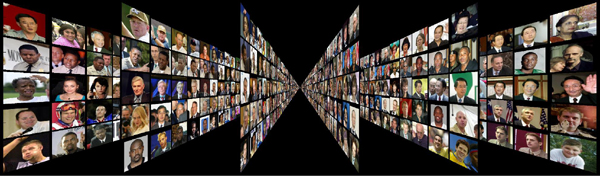
\includegraphics[width=.9\linewidth]{lfiw.jpg}
\end{center}
\vfill
\footnotesize
{\color{blue} \url{http://vis-www.cs.umass.edu/lfw/}} 
\end{frame}


\begin{frame}{MegaFace}
\begin{itemize}
	\item 4.7 миллионов фотографий
	\item Около 700 тысяч человек
	\item В среднем 7 фото на человека
\end{itemize}
\begin{center}
	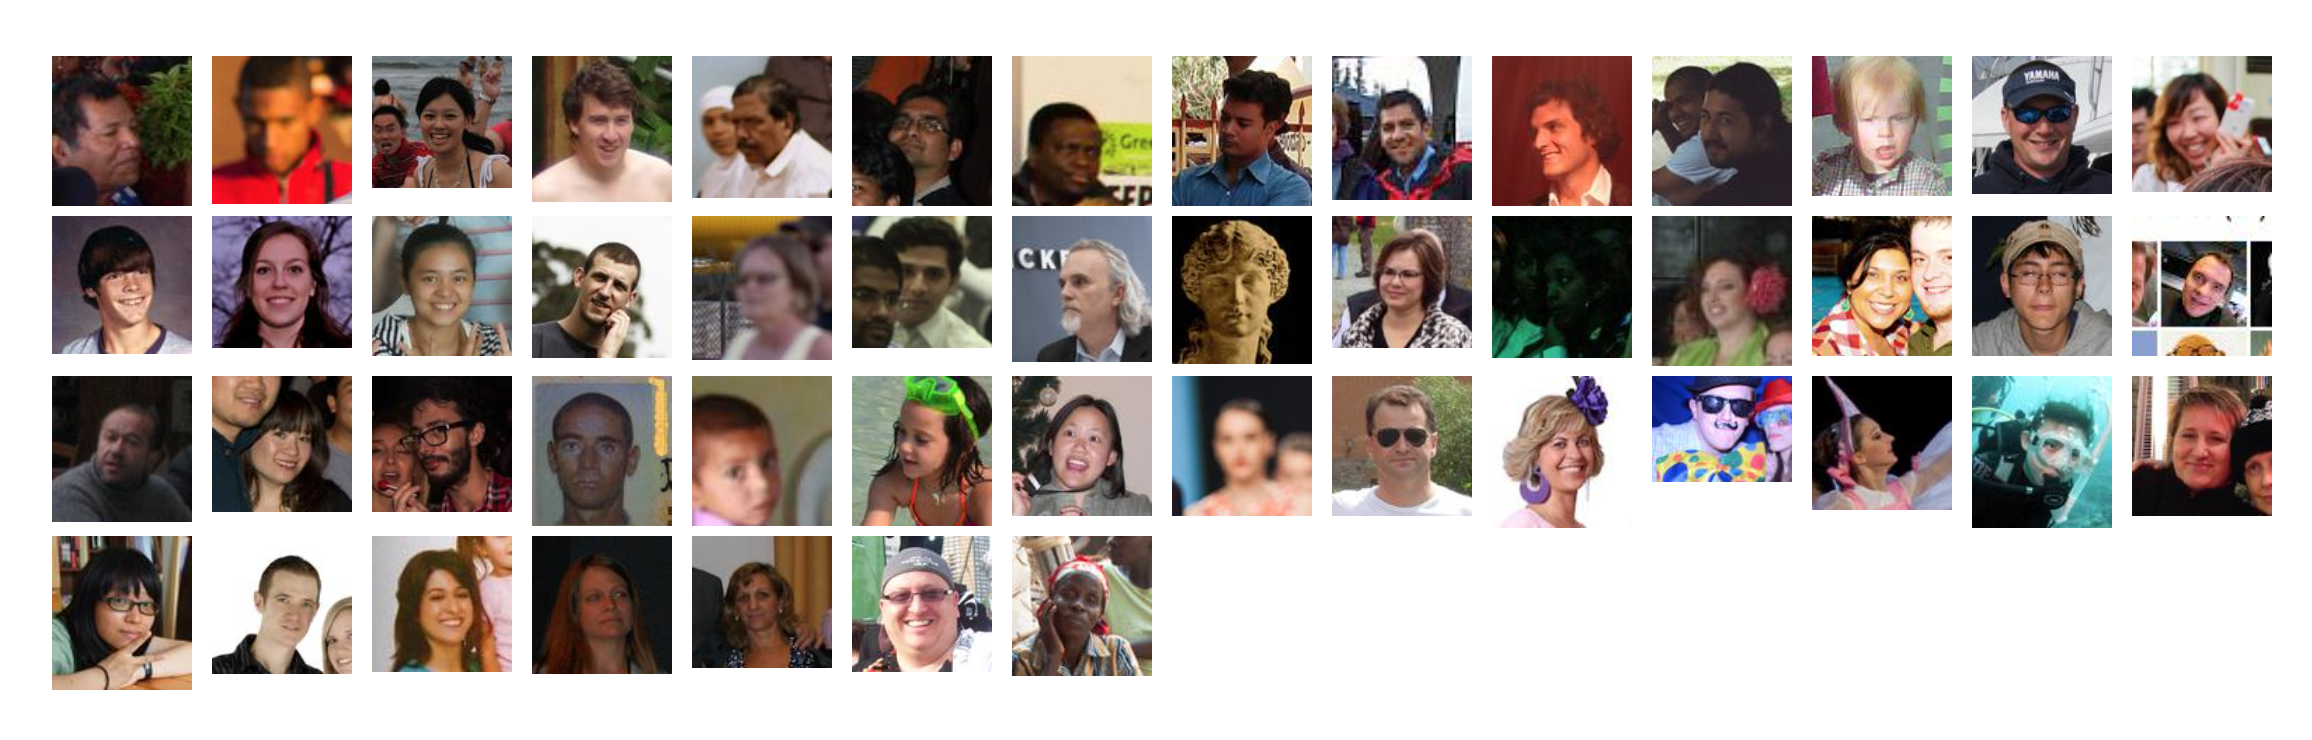
\includegraphics[width=.9\linewidth]{megaface.png}
\end{center}
\vfill
\footnotesize
{\color{blue} \url{http://megaface.cs.washington.edu/}} 
\end{frame}


\begin{frame}{Дообучение (Transfer learning)}
\begin{center}
	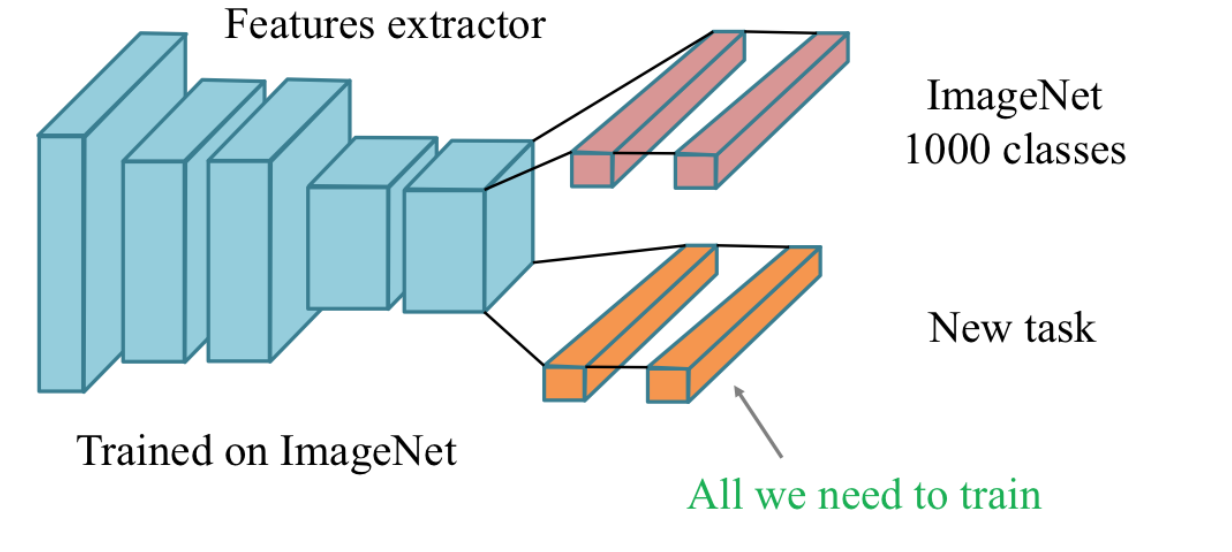
\includegraphics[width=.8\linewidth]{transfer_learning2.png}
\end{center}
\end{frame}


\begin{frame}{Дообучение (Transfer learning)}
\begin{wideitemize}
	\item Если данных совсем мало
	\item Берём модель из другой задачи
	\item Заменяем последний слой на слой с нужным числом выходов
	\item Обучаем только его
	\item По сути, это обучение линейной модели на эмбединге картинки
	\item Иногда приходится дообучать часть экстрактора эмбедингов
\end{wideitemize}
\end{frame}


\begin{frame}{DeepFace (2014)}
\begin{center}
	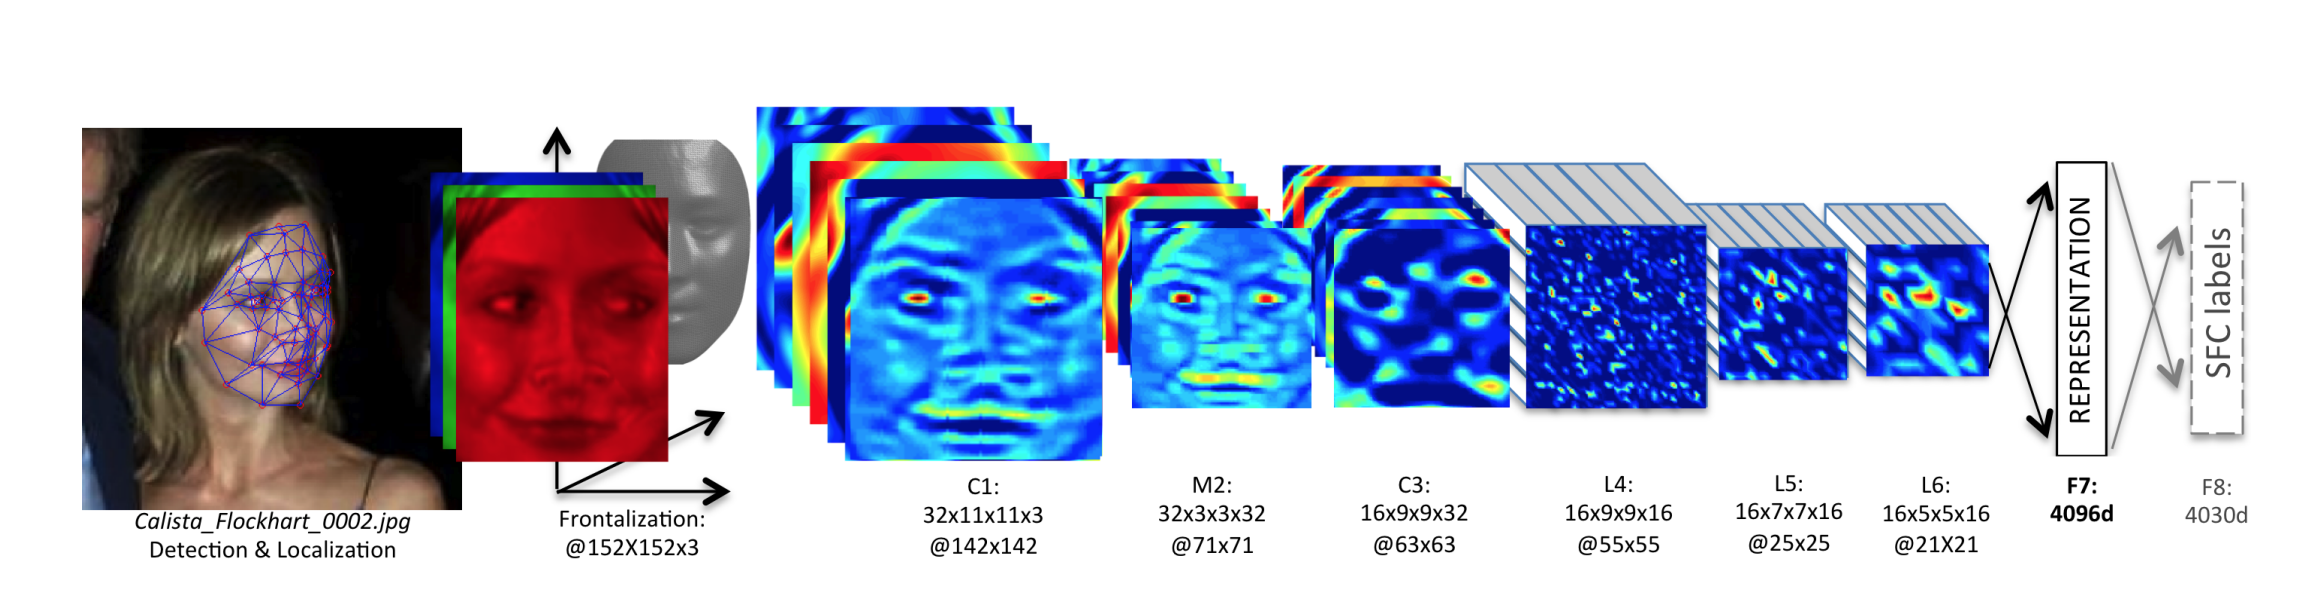
\includegraphics[width=.95\linewidth]{deepface.png}
\end{center}
\vfill
\footnotesize
{\color{blue} \url{https://www.cs.toronto.edu/~ranzato/publications/taigman_cvpr14.pdf}} 
\end{frame}


\begin{frame}{DeepFace (2014)}
\begin{wideitemize}
	\item Обучаем некоторую архитектуру для классификации (число
	классов = число людей в данных)
	\item Используем выходы предпоследнего слоя как признаковое
	описание изображения
	\item Признаки нормализуются (чтобы норма была единичной)
	\item Считаем близость векторов по какой-нибудь метрике
	\item Можно сравнить расстояние с порогом, чтобы идентифицировать
	человека
\end{wideitemize}
\vfill
\footnotesize
{\color{blue} \url{https://www.cs.toronto.edu/~ranzato/publications/taigman_cvpr14.pdf}} 
\end{frame}


\begin{frame}{FaceNet}
\begin{itemize}
	\item Зачем делать так сложно? Почему бы сразу не обучать
	представления изображений так, чтобы фотографии одного человека имели близкие представления?
\end{itemize}
\vfill
\footnotesize
{\color{blue} \url{https://arxiv.org/pdf/1503.03832.pdf}} 
\end{frame}


\begin{frame}{FaceNet}
\begin{itemize}
	\item Нейросеть нужно \alert{умолять обучиться,} батчи  формируем специально так, чтобы в них были и одинаковые и разные люди
\end{itemize}
\begin{center}
	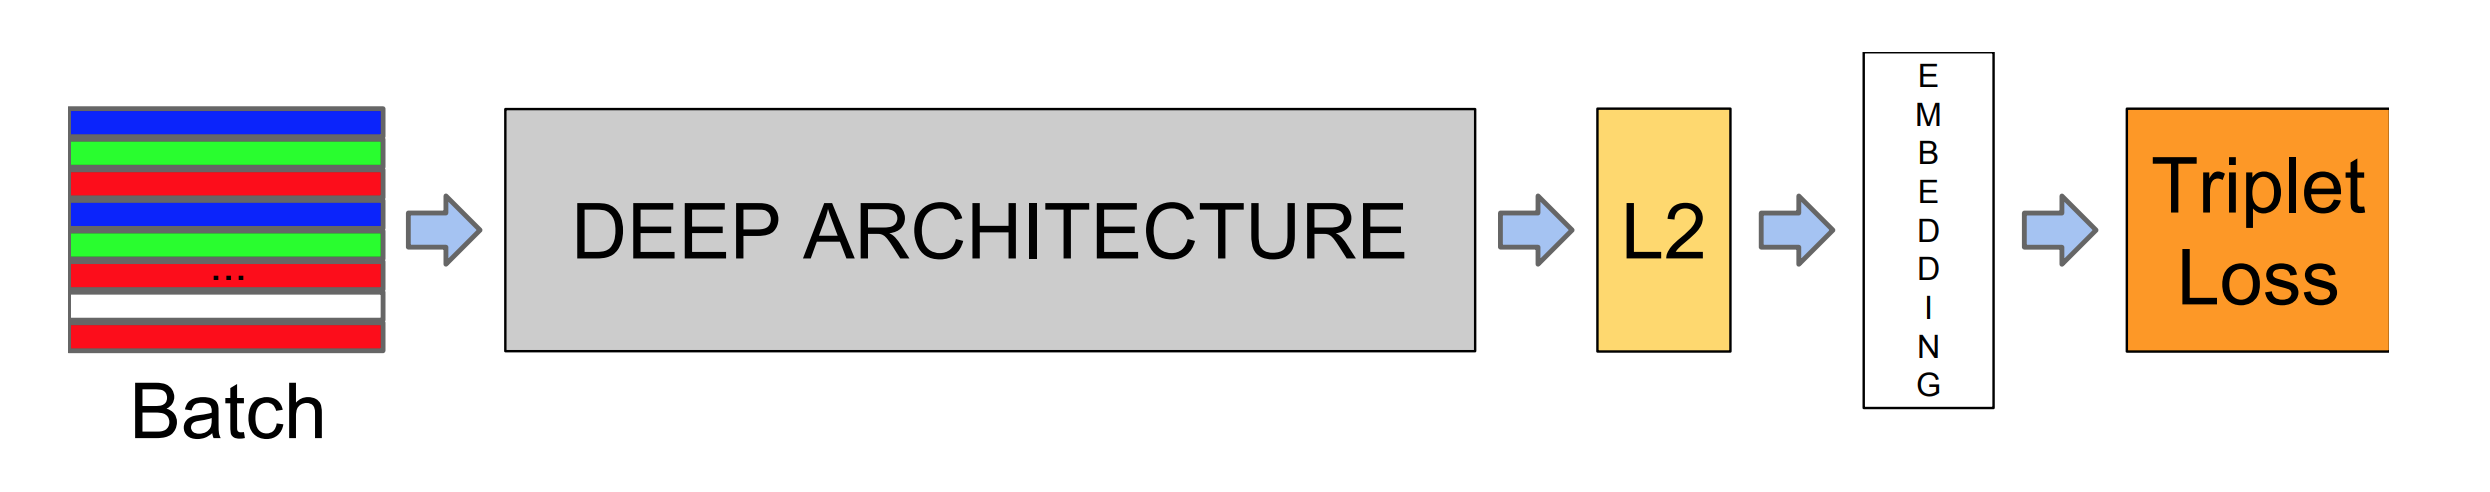
\includegraphics[width=.9\linewidth]{facenet_model.png}
\end{center}
\vfill
\footnotesize
{\color{blue} \url{https://arxiv.org/pdf/1503.03832.pdf}} 
\end{frame}


\begin{frame}{Triplet loss}
\begin{center}
	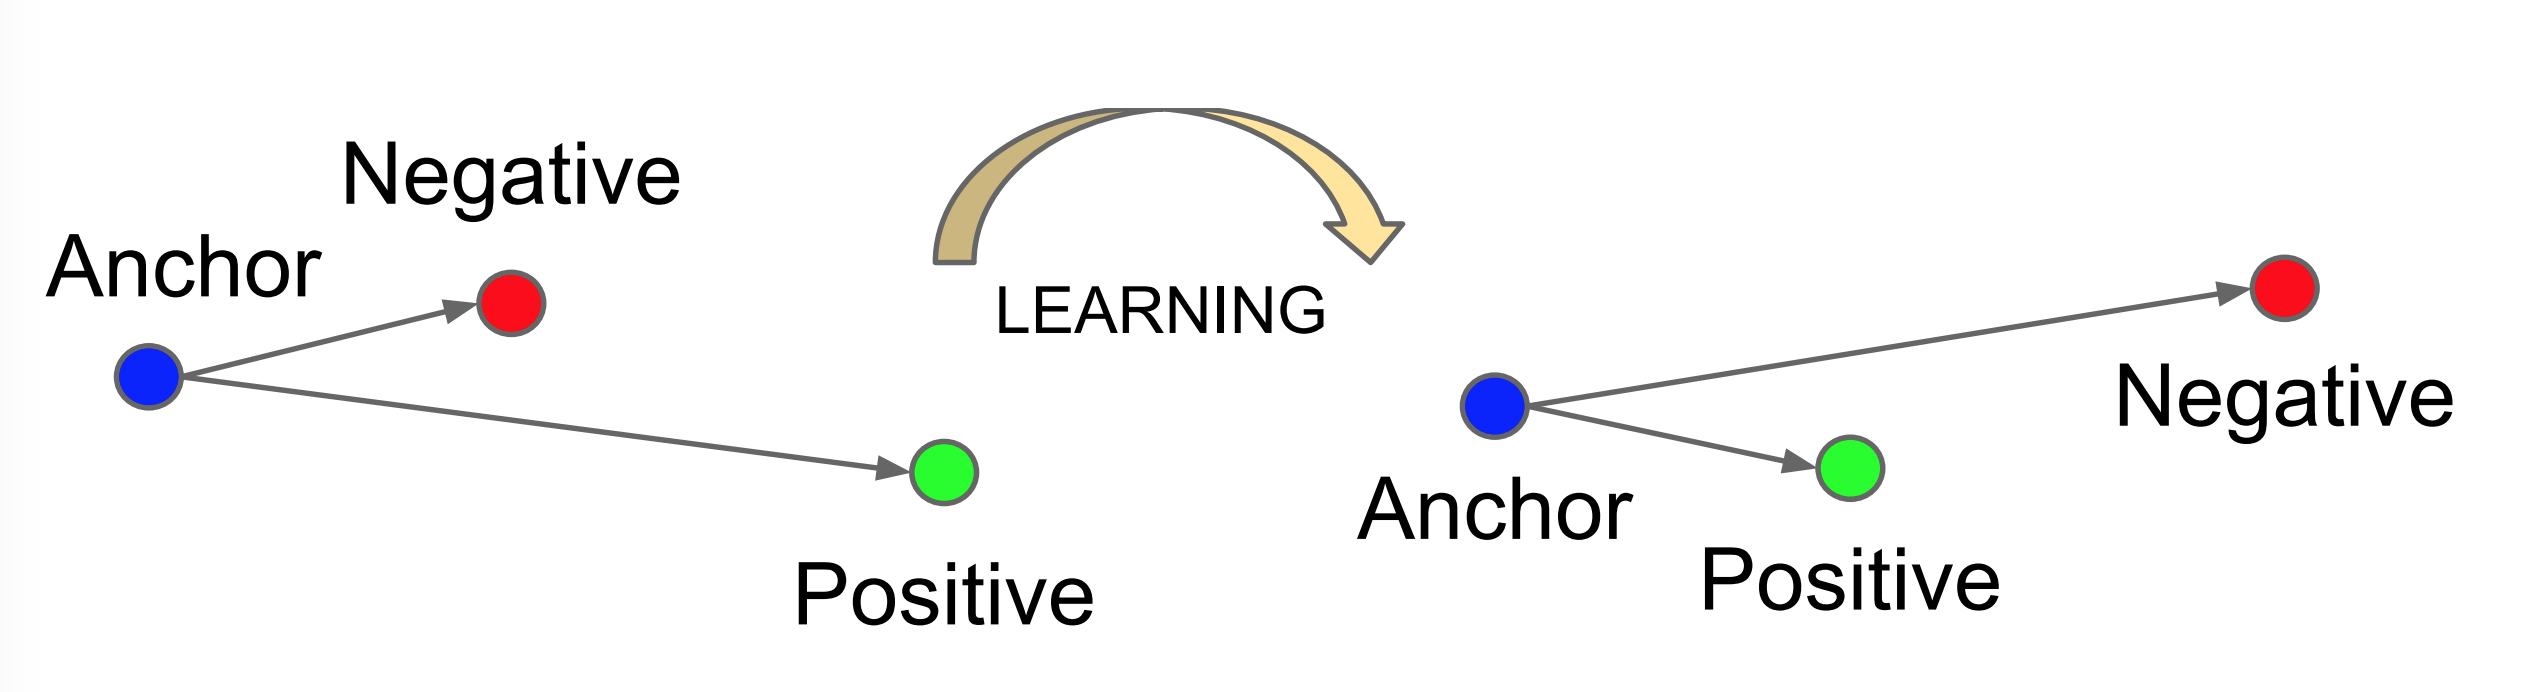
\includegraphics[width=.85\linewidth]{triplet_loss.png}
\end{center}
\[
\sum_{i=1}^N  ReLu( ||f(x_i^a) - f(x_i^p)||^2_2 - ||f(x_i^a) - f(x_i^n)||^2_2 + \alpha )
\]
\vfill
\footnotesize
{\color{blue} \url{https://arxiv.org/pdf/1503.03832.pdf}} 
\end{frame}


\begin{frame}{Triplet loss}
\begin{wideitemize}
	\item Важно правильно выбирать триплеты
	\item Обычно: выбираем positive и ищем semi-hard negatives
	\item Обычно в имлиментации любой современной нейронки есть куча костылей, вставленных чтобы она действительно обучалась
\end{wideitemize}
\[
||f(x_i^a) - f(x_i^p)||^2_2  <  ||f(x_i^a) - f(x_i^n)||^2_2  
\]
\vfill
\footnotesize
{\color{blue} \url{https://arxiv.org/pdf/1503.03832.pdf}} 
\end{frame}


\begin{transitionframe}
	\begin{center}
		\Huge  Обучение без учителя
	\end{center}
\end{transitionframe}


\begin{frame}{Представления изображений}
\begin{center}
	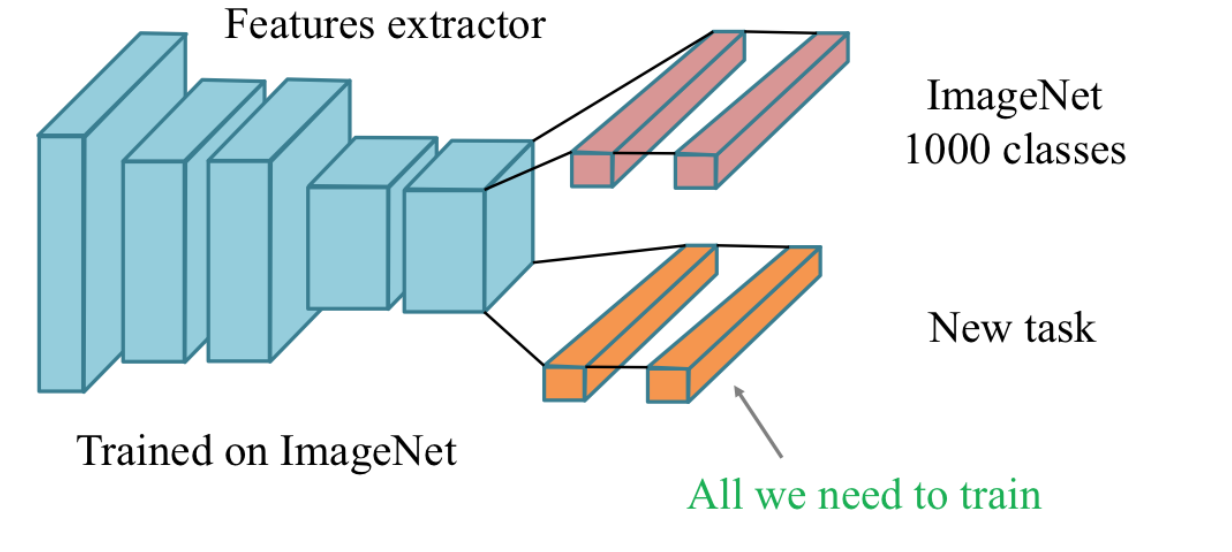
\includegraphics[width=.8\linewidth]{transfer_learning2.png}
\end{center}
\end{frame}


\begin{frame}{Представления изображений}
\begin{wideitemize}
	\item Выход предпоследнего полносвязного слоя — хорошее
	представления картинки
	\item Но для его обучения нужны изображения с разметкой
	\item Может, получится строить такие представления и без разметки?	
\end{wideitemize}
\end{frame}


\begin{frame}{Автокодировщики}
	\begin{center}
		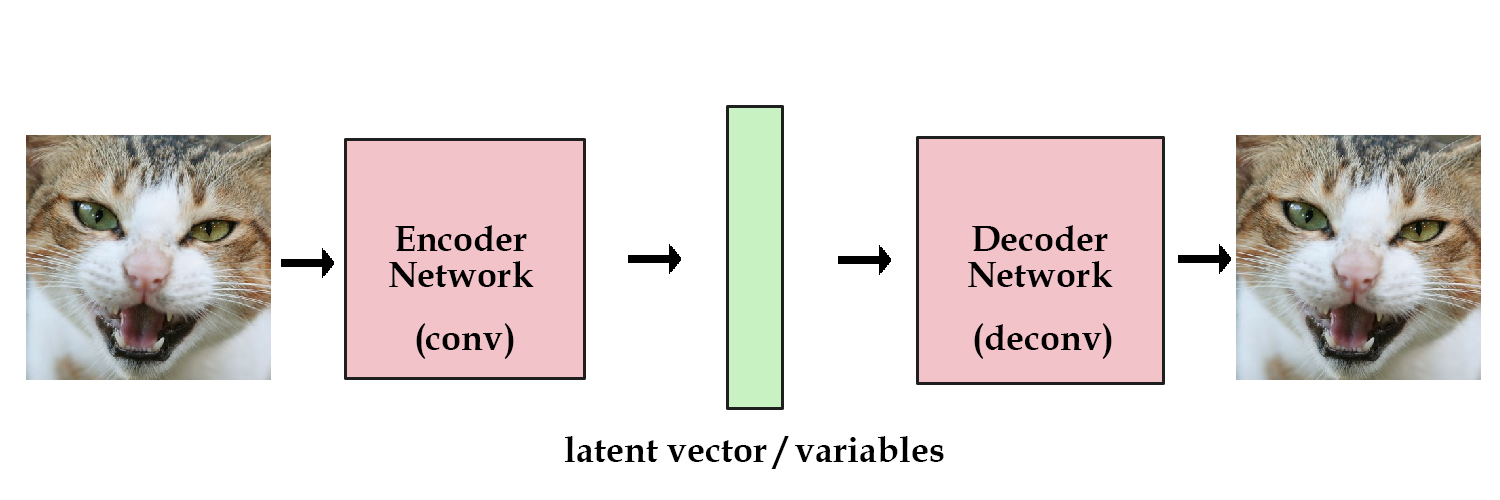
\includegraphics[width=.9\linewidth]{autoencoder.png}
	\end{center}
\end{frame}


\begin{frame}{Автокодировщики}
\begin{center}
	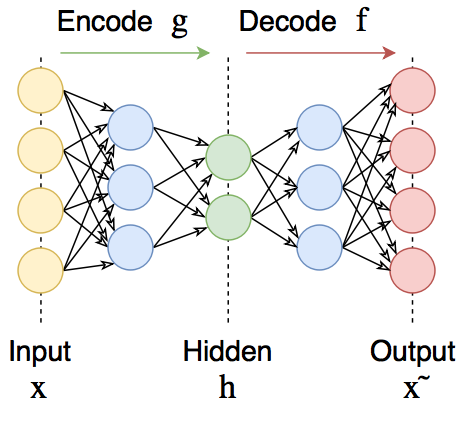
\includegraphics[width=.42\linewidth]{auto.png}
\end{center} \pause
\[
\frac{1}{n} \sum_{i=1}^n L(x_i, f(g(x_i))) \to \min 
\]
\end{frame}


\begin{frame}{Пример сжатия}
	\begin{center}
		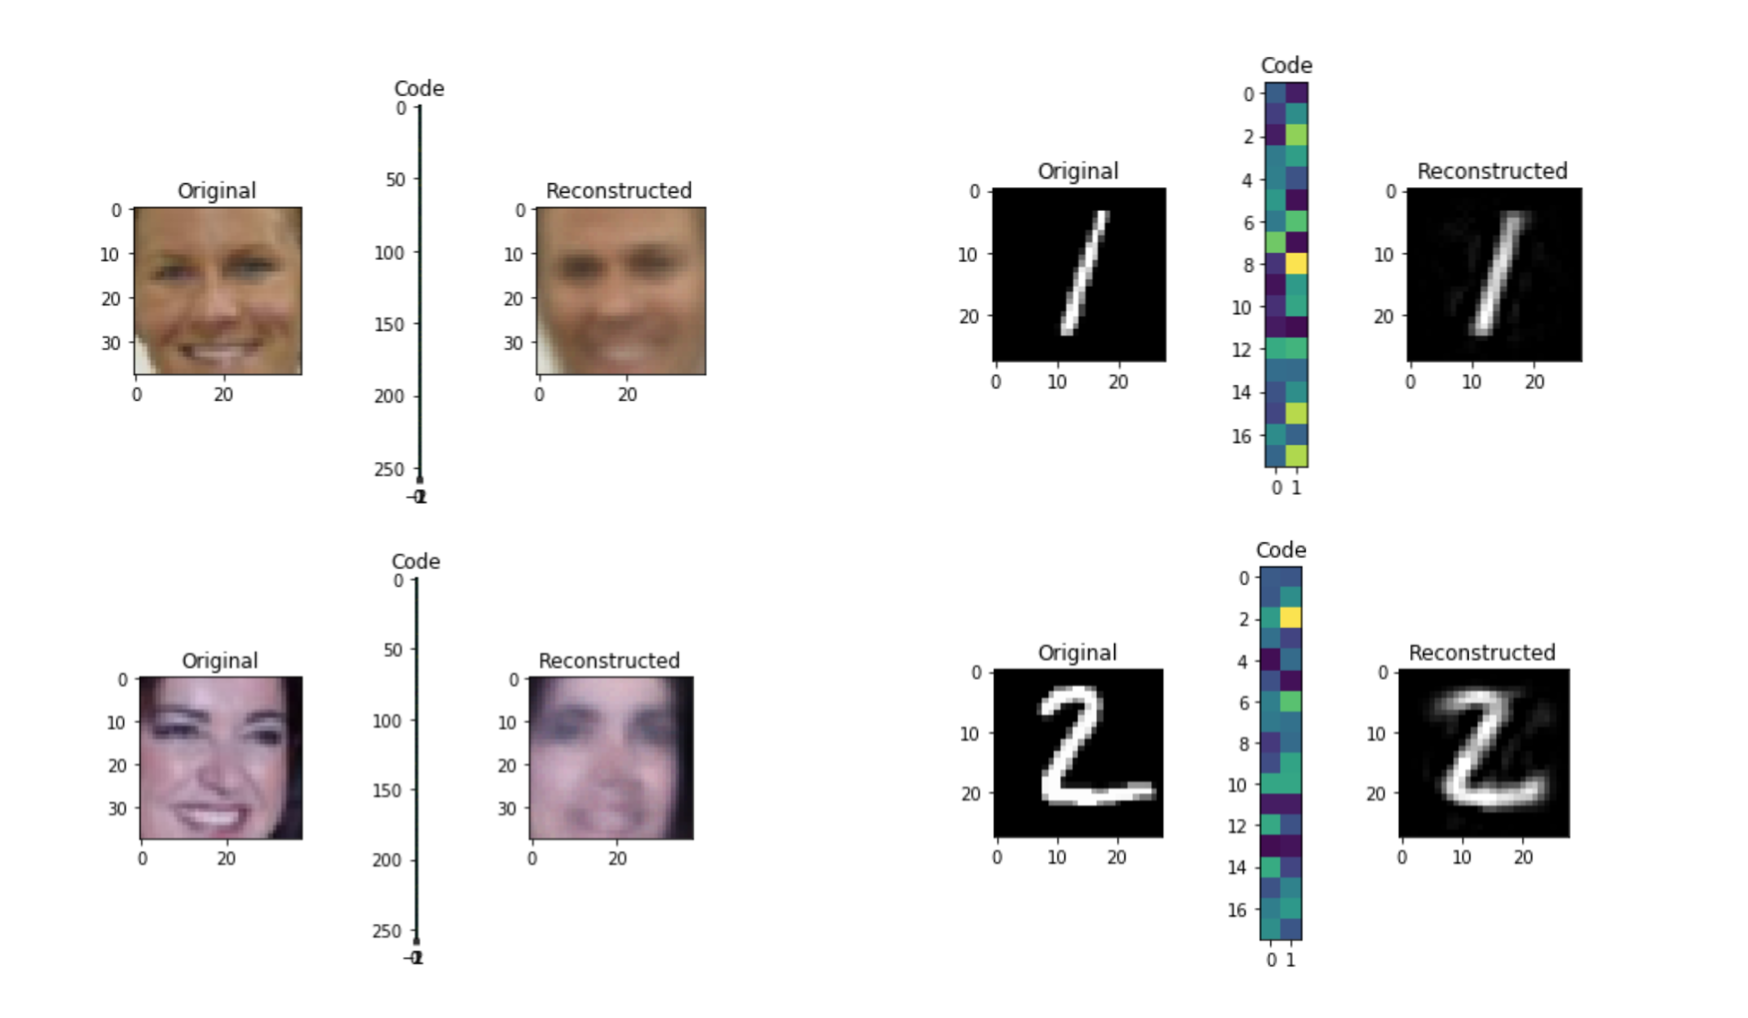
\includegraphics[width=.8\linewidth]{ato_enc.png}
	\end{center}
\end{frame}

\begin{frame}{Зачем это всё?}
\begin{wideitemize}
	\item  Сжатие данных (нелинейных аналог PCA)
	\item  Очистка картинки от шума
	\item  Поиск похожих изображений
	\item  Трансформация изображений
	\item  Генерация изображений
\end{wideitemize}
\end{frame}


\begin{frame}{Автокодировщики}
\begin{wideitemize}
	\item  Понижают размерность, исходная картинка восстанавливается с потерями
	\item  Основная ценность — эмбединг из булочного горлышка, хочется чтобы он получился максимально качественным
	\item  Наша архитектура сильно переобучается под выборку, для новых лиц работает хуже
	\item  Нужна регуляризация, которая позволит извлекать смысл, а не восстанавливать пиксели в точности (фон тоже запоминается)
\end{wideitemize}
\end{frame}


\begin{frame}{Что находит нейросеть... опять ...}
	\begin{center}
		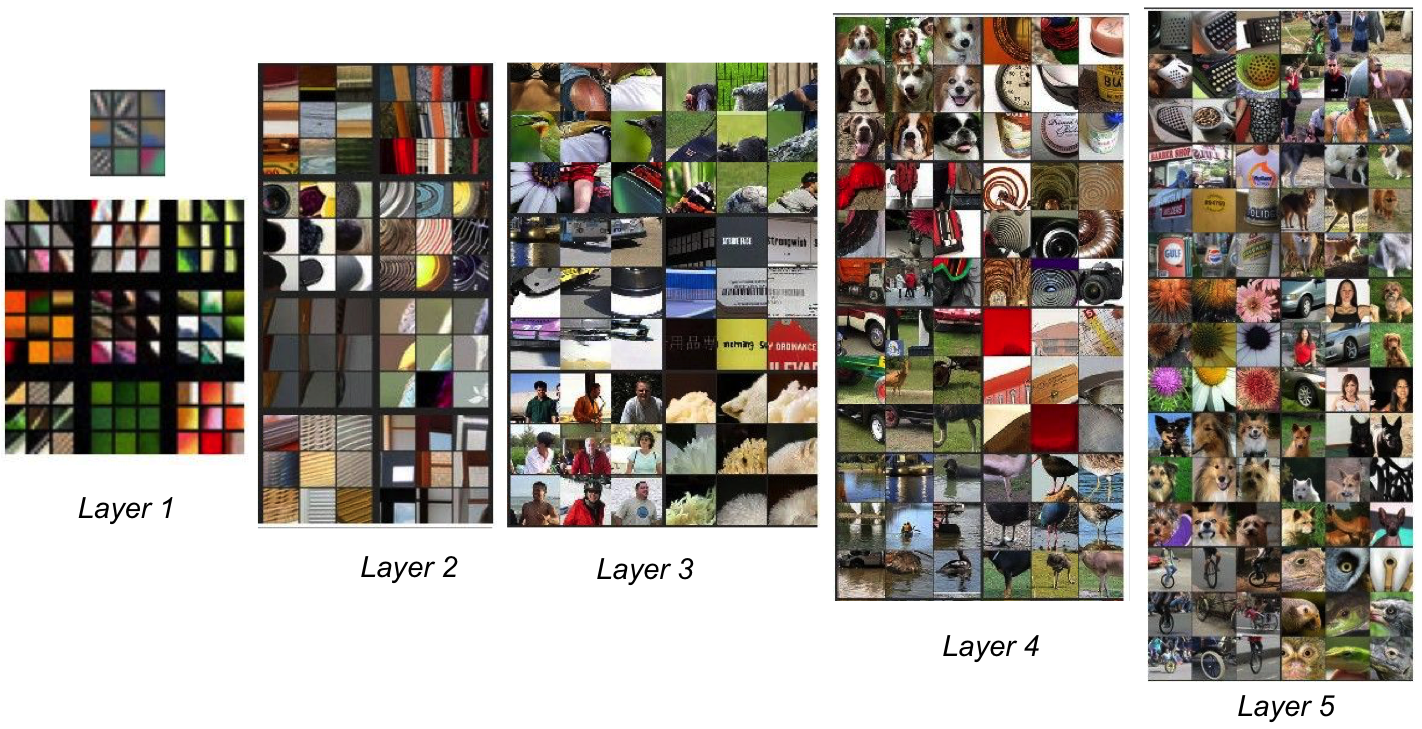
\includegraphics[width=.85\linewidth]{cnn_vis.png}
	\end{center}
\end{frame}


\begin{frame}{Perceptual loss}
	\begin{center}
		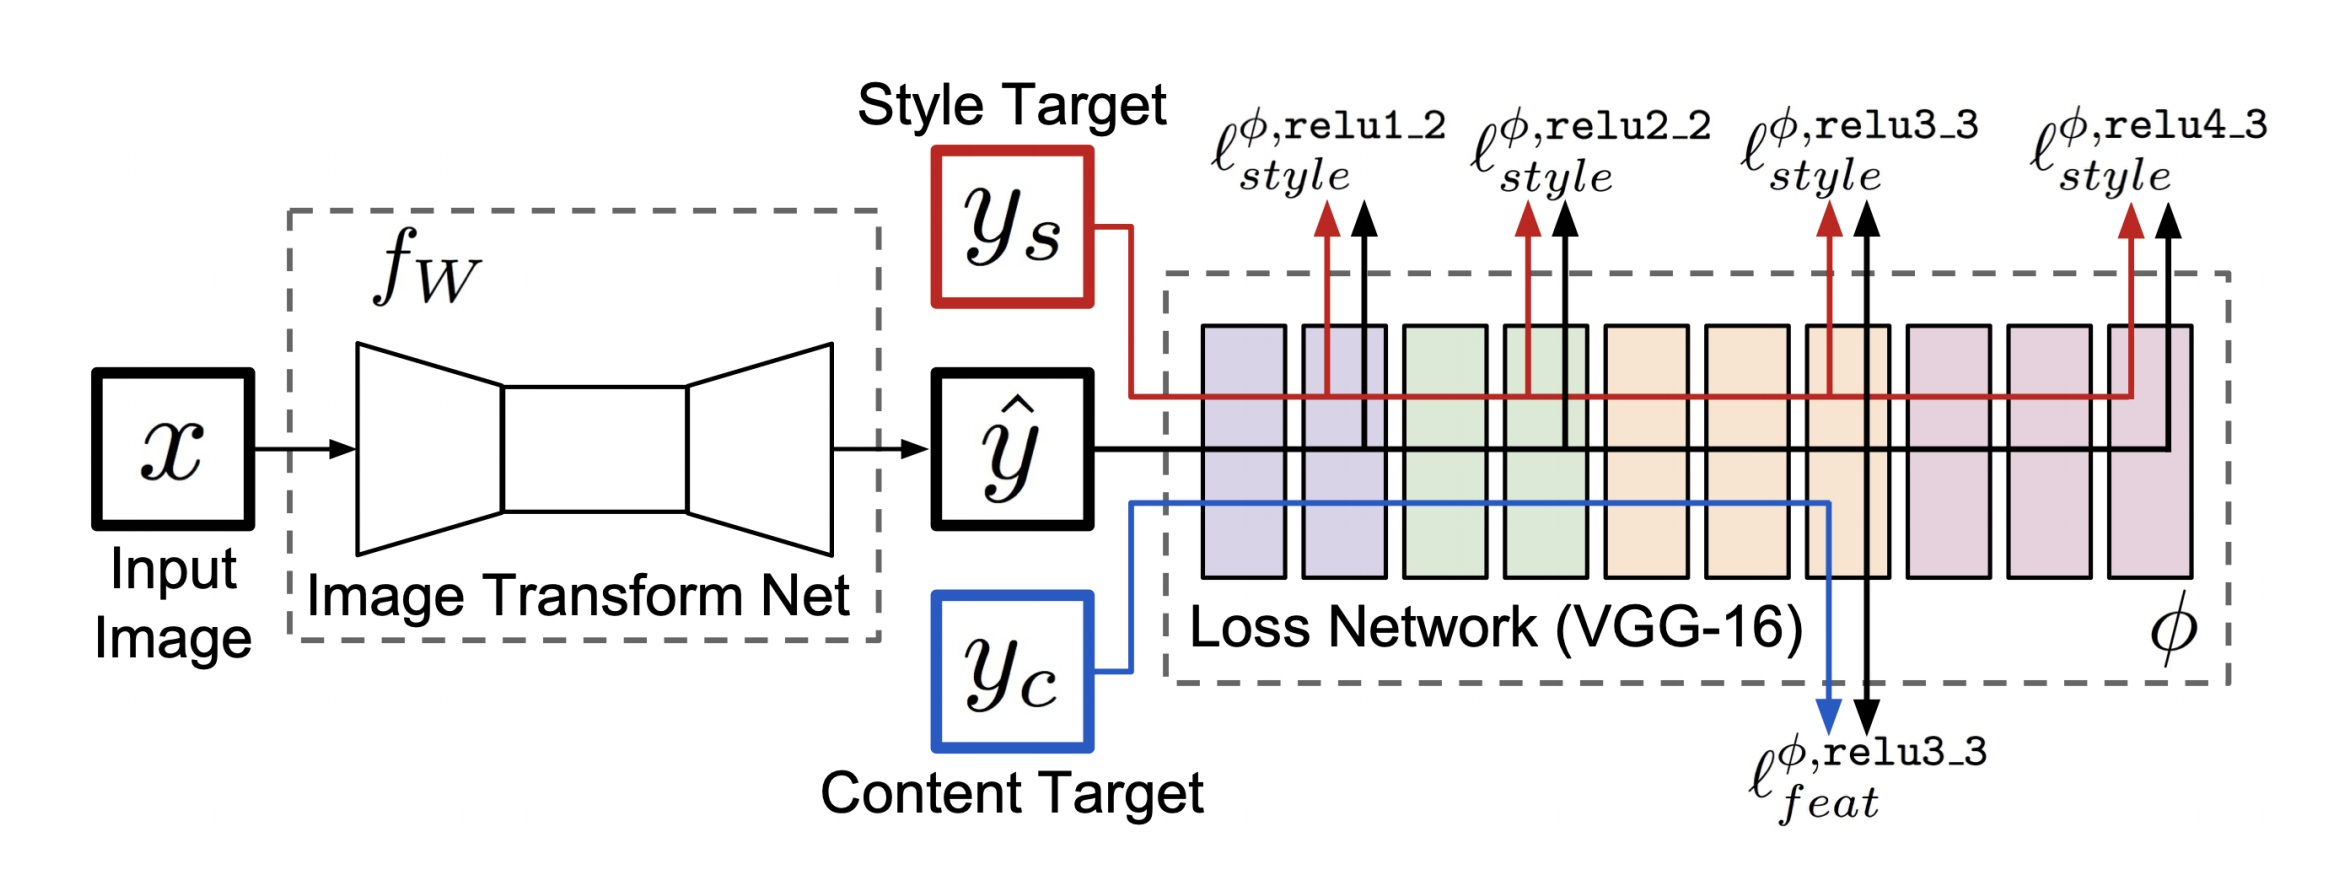
\includegraphics[width=.8\linewidth]{perceptual_loss.png}
	\end{center}
	\vfill
	\footnotesize
	{\color{blue} \url{https://arxiv.org/pdf/1603.08155.pdf}} 
\end{frame}


\begin{frame}{Perceptual loss}
\begin{wideitemize}
	\item  Чем глубже слой, тем осмысленнее образы
	\item  Ранние слои во многом определяют стиль картинки
	\item  Можно измерять расстояния между выходами свёрточных слоёв картинок
	\item  Это поможет сохранить смысл и сделать эмбединг более осмысленным
\end{wideitemize}
	\vfill
\footnotesize
{\color{blue} \url{https://arxiv.org/pdf/1603.08155.pdf}} 
\end{frame}


\begin{frame}{Denoising autoencoder}
\begin{center}
	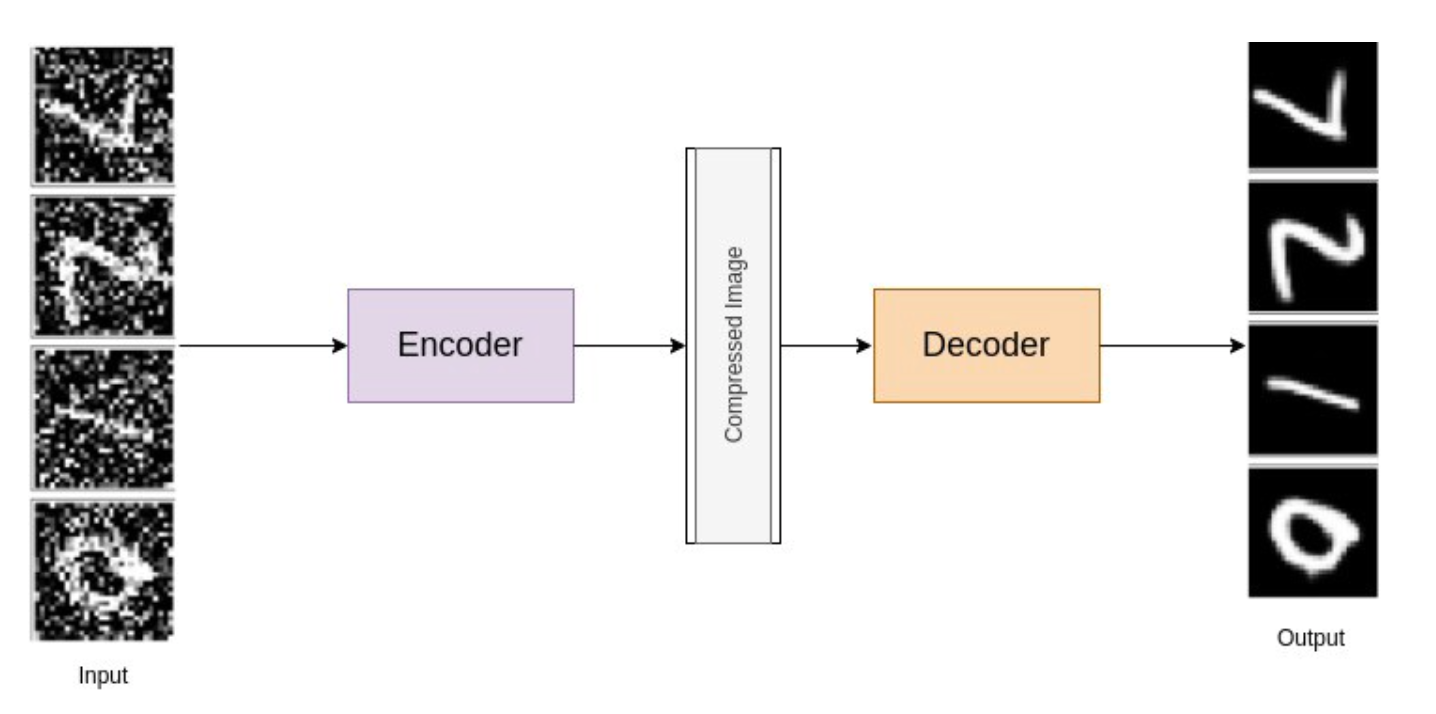
\includegraphics[width=.8\linewidth]{denoise.png}
\end{center}
\vfill
\footnotesize
{\color{blue} \url{https://medium.com/@garimanishad/reconstruct-corrupted-data-using-denoising-autoencoder-python-code-aeaff4b0958e} \newline \url{https://www.cs.toronto.edu/~larocheh/publications/icml-2008-denoising-autoencoders.pdf} } 
\end{frame}


\begin{frame}{Morphing faces}
\begin{center}
	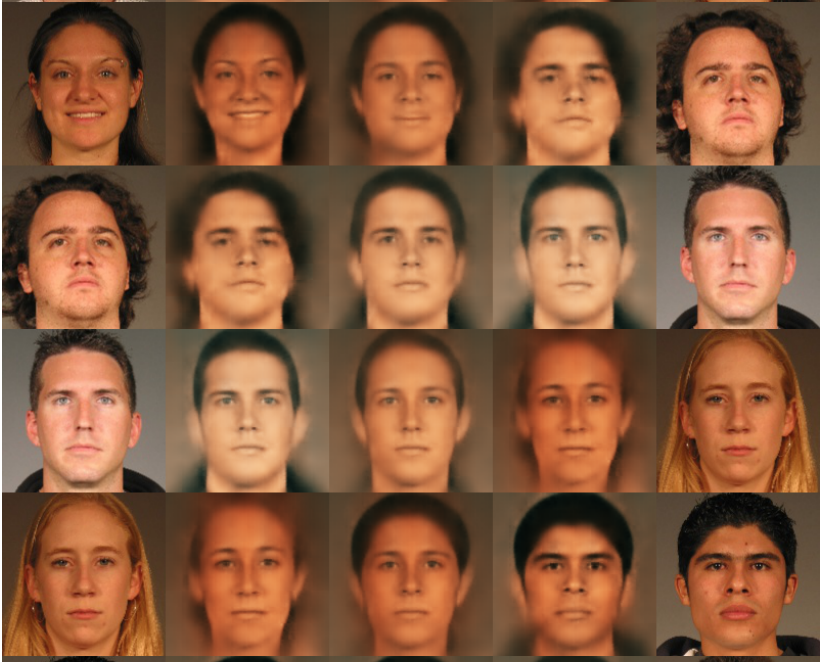
\includegraphics[width=.5\linewidth]{morth.png}
\end{center}
\vfill
\footnotesize
{\color{blue} \url{http://essay.utwente.nl/81372/1/Heuver_MA_EEMCS.pdf}  } 
\end{frame}


\begin{frame}{Morphing faces}
\begin{center}
	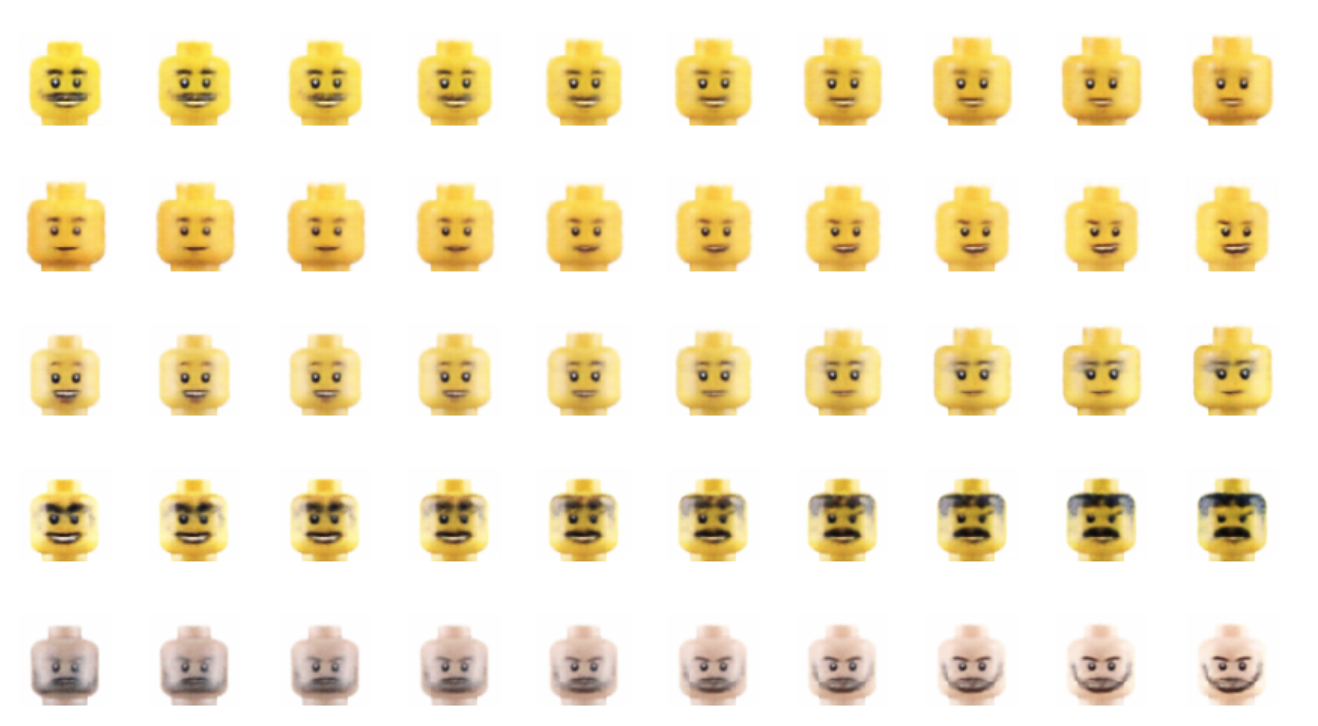
\includegraphics[width=.9\linewidth]{lego.png}
\end{center}
\vfill
\footnotesize
{\color{blue} \url{https://www.echevarria.io/blog/lego-face-vae/index.html}  } 
\end{frame}




\begin{frame}{Саморегуляция выборки}
%\begin{center}
%	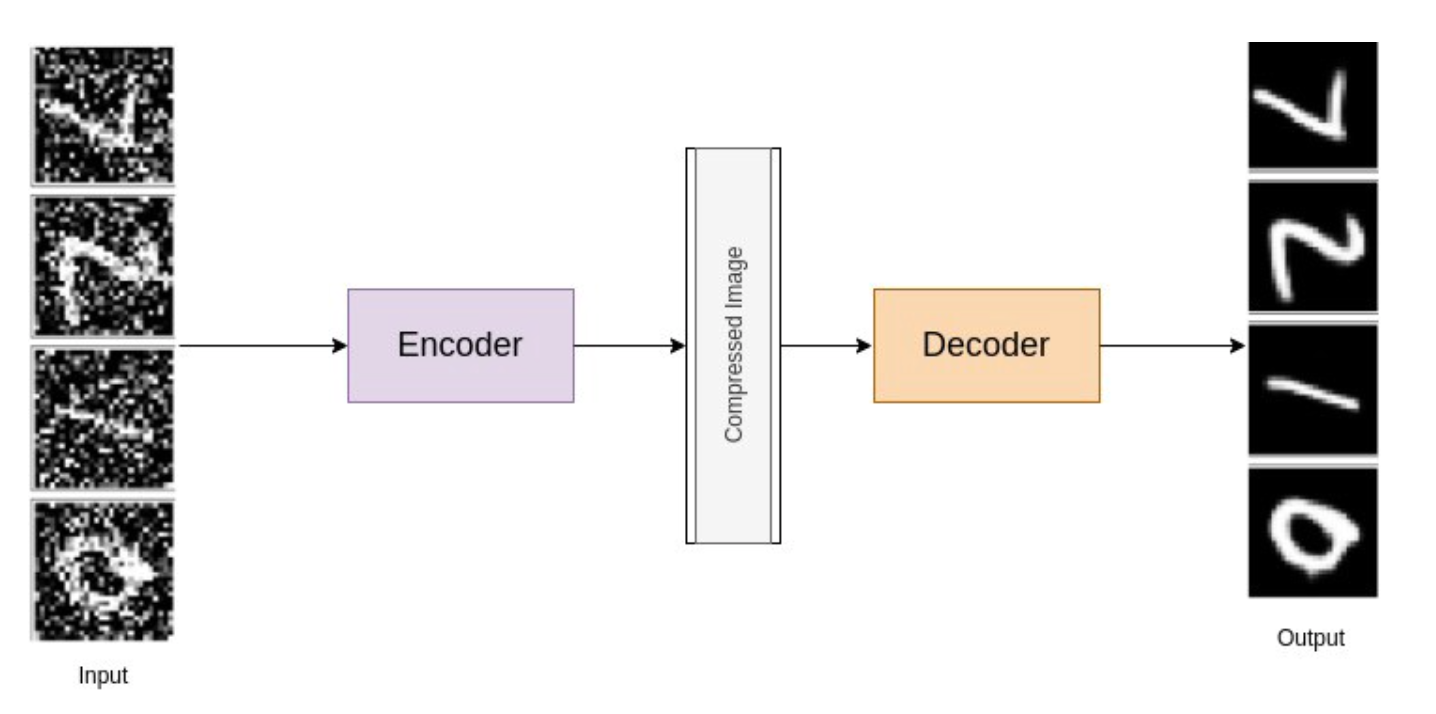
\includegraphics[width=.8\linewidth]{denoise.jpeg}
%\end{center}
\vfill
\footnotesize
{\color{blue} \url{https://nplus1.ru/news/2019/01/28/debiasing-faces}  } 
\end{frame}





\begin{transitionframe}
	\begin{center}
		\Huge  GAN
	\end{center}
\end{transitionframe}


\begin{frame}
\begin{center}
	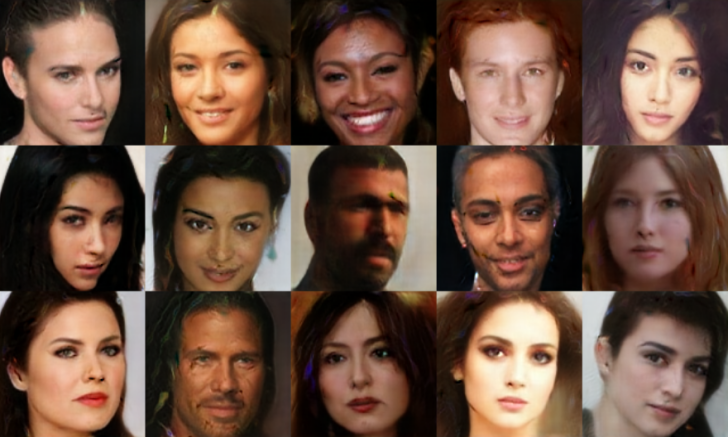
\includegraphics[width=.8\linewidth]{face_teaser.png}
\end{center}
\vfill
\footnotesize
{\color{blue} \url{https://thispersondoesnotexist.com} \\ 
\url{https://arxiv.org/pdf/1812.04948.pdf}}
\end{frame}


\begin{frame}
\begin{center}
	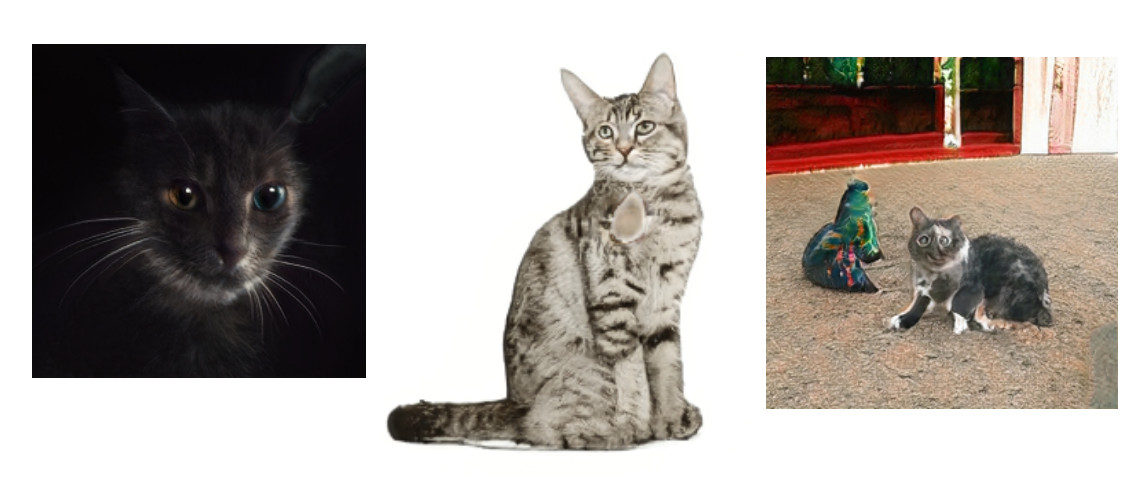
\includegraphics[width=.9\linewidth]{cat_teaser.png}
\end{center}
\vfill
\footnotesize
{\color{blue} \url{https://thiscatdoesnotexist.com}}
\end{frame}


\begin{frame}{Генеративные сети}
\begin{center}
	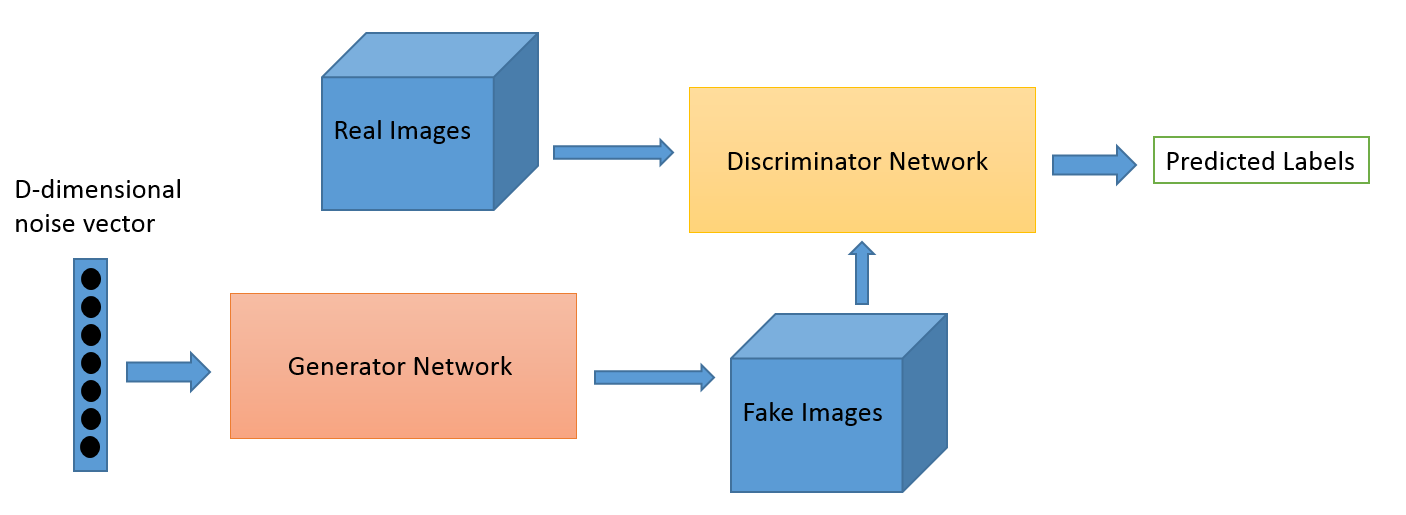
\includegraphics[width=.95\linewidth]{gan1.png}
\end{center}
\vfill
\footnotesize
{\color{blue} \url{https://arxiv.org/abs/1406.2661}}
\end{frame}


\begin{frame}{Генеративные сети}
\begin{wideitemize}
	\item   Две нейронных сетки 
	\item   \alert{Генератор}  сэмплит из какого-то случайного распределения вектора и пытается переработать их в картинки 
	\item   \alert{Дискриминатор}  получает на вход сгенерированные картинки и настоящие, пытается отличить реальные данные от подделки   
\end{wideitemize}
\end{frame}


\begin{frame}{Генеративные сети}
\begin{center}
	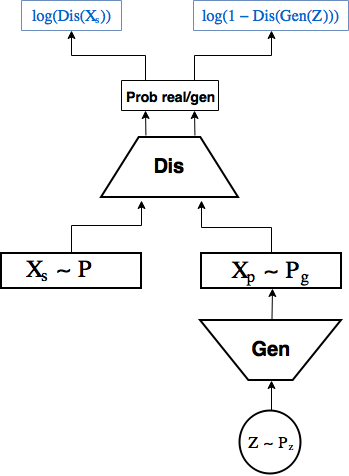
\includegraphics[width=.35\linewidth]{gan_1.png}
\end{center}
\end{frame}


\begin{frame}{Обучение сеток}
\begin{center}
	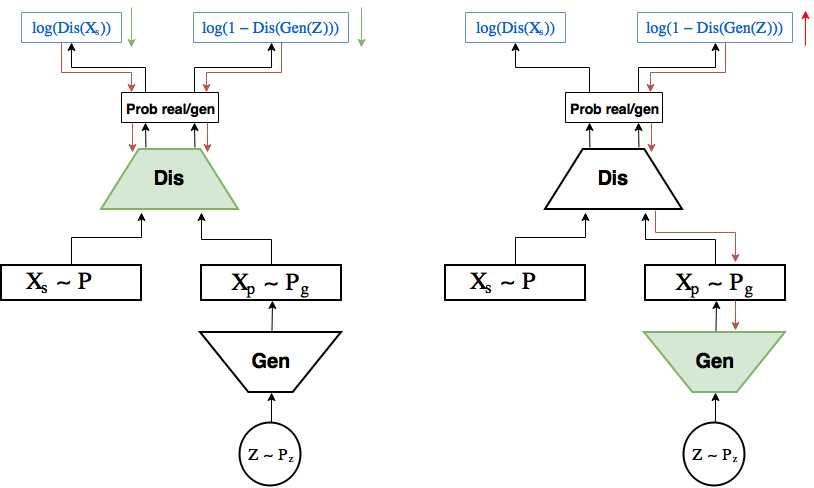
\includegraphics[width=.8\linewidth]{gan_2.png}
\end{center}
\end{frame}


\begin{frame}{Обучение сеток}
\begin{wideitemize}
	\item   Обучение сеток происходит поэтапно 
	\item   Сначала несколько шагов дискриминатор учится различать правду от лжи, минимизируется  
	
	\[ L_D =  - y_i \cdot \ln \hat p_i - (1 - y_i) \cdot \ln (1 - \hat p_i)  \to \min_{D} \]  \pause 
	
	\item   После происходит один шаг обучения генератора, он пытается заставить дискриминатор ошибаться и максимизирует значение ошибки на ложных картинках
	
	\[ 
	L_G = - \ln (1 - \hat p_i)  \to \max_{G}
	\]
\end{wideitemize}
\end{frame}


\begin{frame}{Обучение сеток}
\begin{center}
	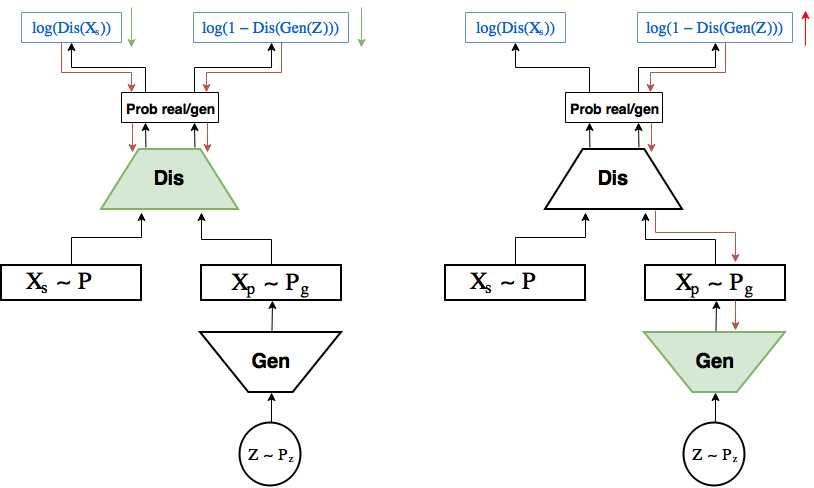
\includegraphics[width=.8\linewidth]{gan_2.png}
\end{center}
\end{frame}


%\begin{frame}{Задача}
%\begin{wideitemize}
%	\item   Если совсем-совсем заниматься формализмом, мы решаем задачу: 
%	
%	\[
%	\min_{G} \max_{D}  E_X (\ln D(X))  + E_Z (\n(1 - D(G(Z)))) 
%	\]   \pause 
%	
%	\item   При заданном генераторе, оптимальный дискриминатор прогнозирует 
%	
%	\[ 
%	D^{*}(X)  = \frac{P(X)}{P_g(X) + P(X)} 
%	\]
%\end{wideitemize}
%\end{frame}
%
%
%\begin{frame}{Оптимальное решение задачи}
%\begin{center}
%	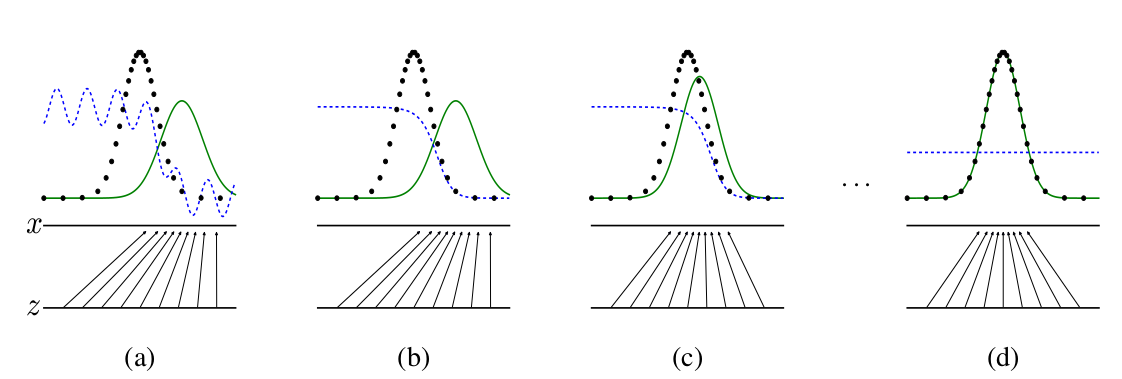
\includegraphics[width=.9\linewidth]{probability.png}
%\end{center}
%\end{frame}

\begin{transitionframe}
	\begin{center}
		\Huge  Собрал, запустил, не работает :( 
	\end{center}
\end{transitionframe}

\begin{frame}{Кекс 1}
\begin{center}
	\begin{columns}[T] % align columns
		\begin{column}{.48\textwidth}
		\centering	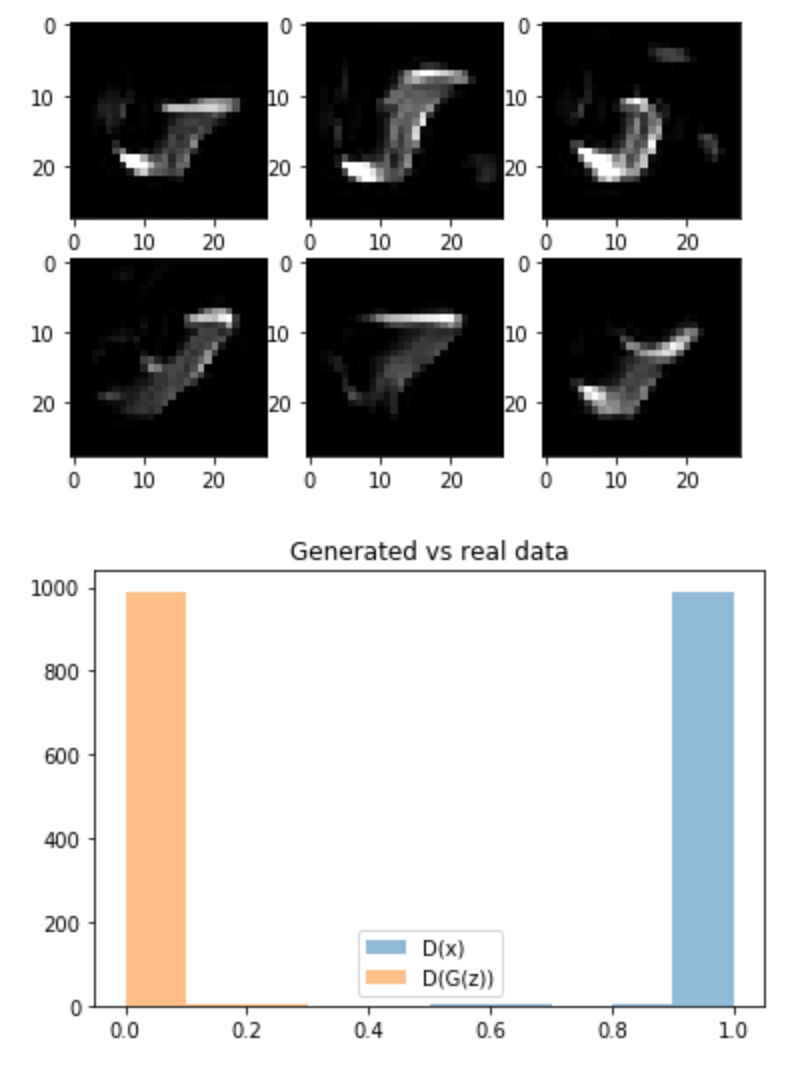
\includegraphics[width=.7\linewidth]{bad2.png}
		\end{column}%
		\begin{column}{.48\textwidth}
		\centering	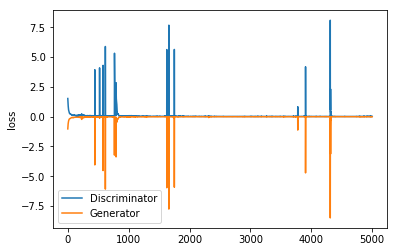
\includegraphics[width=.9\linewidth]{bad1.png}
		\end{column}%	
	\end{columns}
\end{center}
\end{frame}


\begin{frame}{Кекс 2}
\begin{center}
			\centering	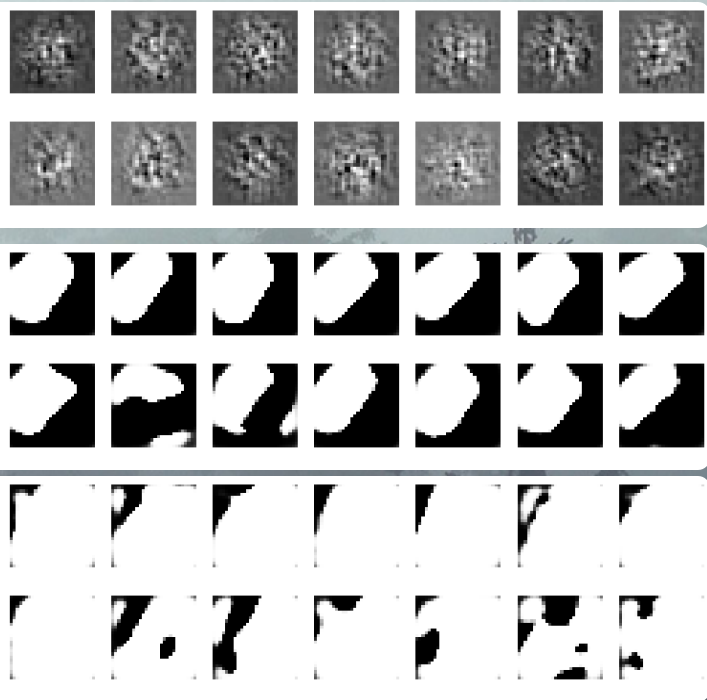
\includegraphics[width=.5\linewidth]{bad3.png}
\end{center}
\end{frame}


\begin{frame}
\begin{center}
	\centering	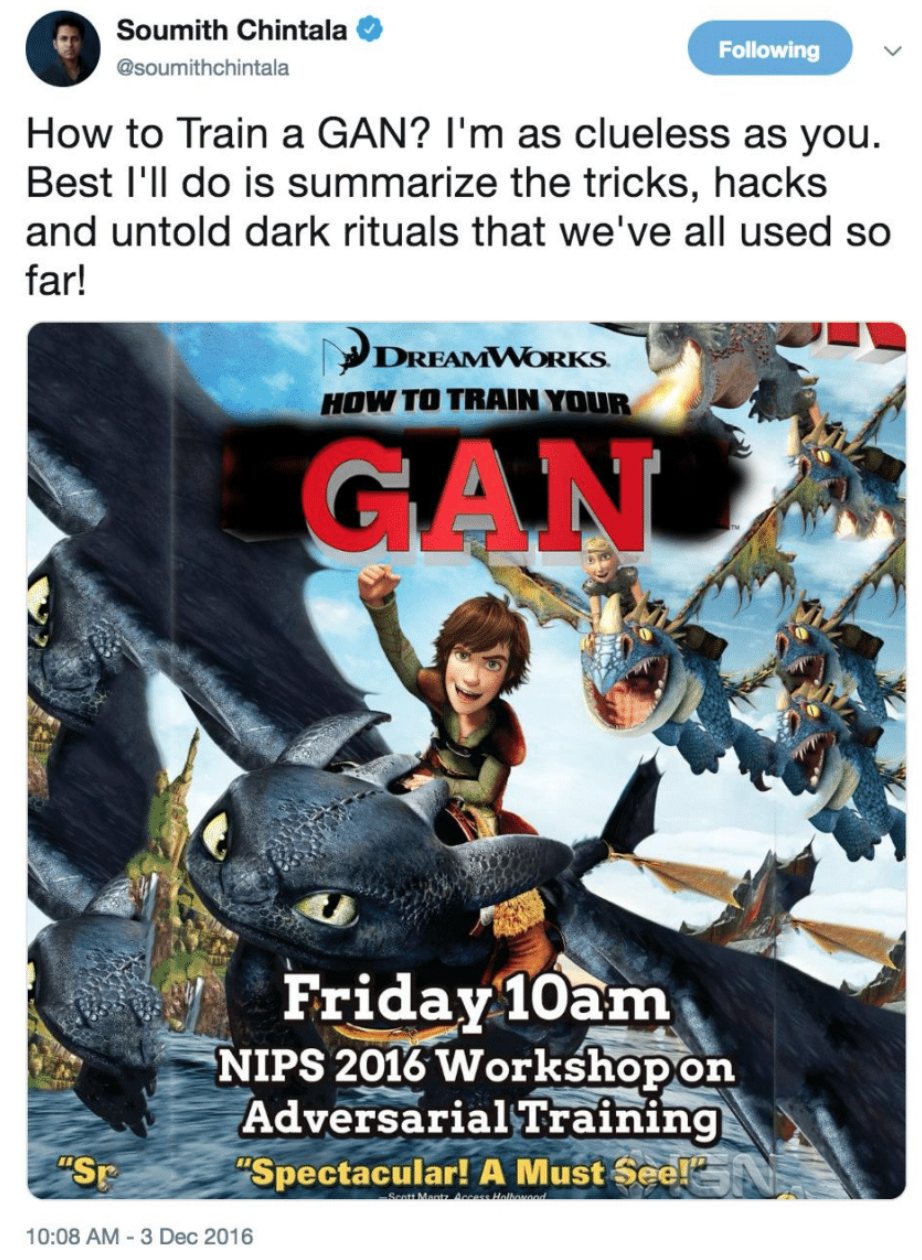
\includegraphics[width=.4\linewidth]{gan_dragon.png}
\end{center}
\end{frame}


\begin{transitionframe}
	\begin{center}
		\Huge  Свёрточные ганы
	\end{center}
\end{transitionframe}


\begin{frame}{Deep Convolutional GAN }
\begin{center}
	\centering	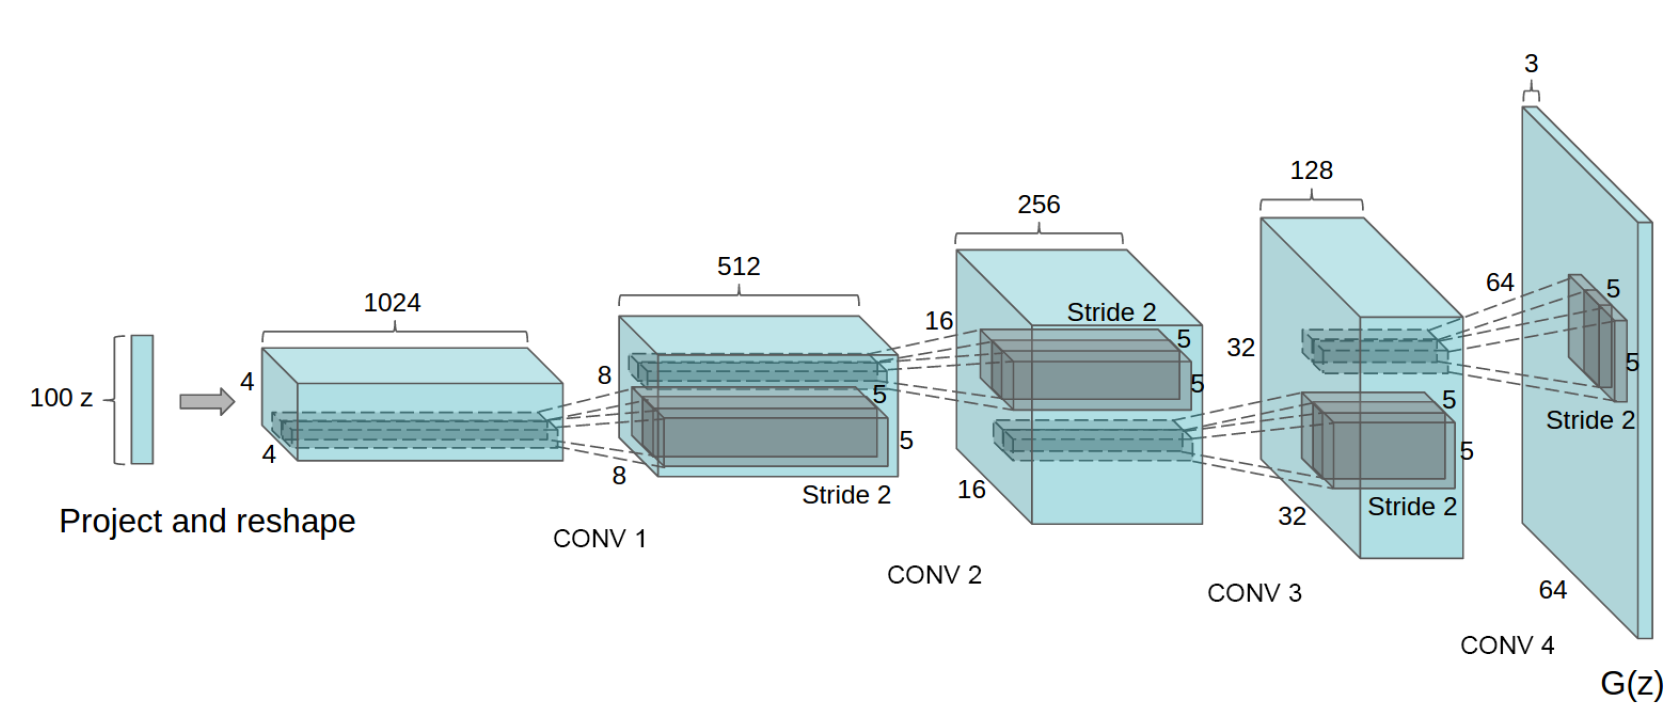
\includegraphics[width=.9\linewidth]{conv_gan.png}
\end{center}
\vfill
\footnotesize
{\color{blue} \url{https://arxiv.org/pdf/1511.06434.pdf}}
\end{frame}

\begin{frame}{Советы для хороших хозяюшек [1]}
\begin{wideitemize}
	\item   Нормализуйте входы на $[-1, 1]$ и на последний слой генератора добавляйте Tanh 
	\item   Сэмплируйте из нормального распределения, а не из равномерного
	\item   Используйте разные BatchNorm  в обеих сетках 
	\item   Можно попробовать использовать разный BatchNorm  для фэйковых и реальных данных 
	\item   Полносвязные слои не очень хорошая мысль, свёрточные — хорошая
\end{wideitemize}
\end{frame}


\begin{frame}{Советы для хороших хозяюшек [2]}
\begin{wideitemize}
\item   Лучше избегать пулинга и делать stridge внутри свёрток 
\item   Если градиенты разряжены, GAN ведёт себя стабильнее,  ReLU и её модификации — хорошая идея 
\item   Зашумляйте реальные данные, чтобы не возникало переобучения
\item   Если в самом начале дискриминатор сильно вырвется вперёд, обучение может заглохнуть
\end{wideitemize}
\vfill
\footnotesize
Ещё советы:  {\color{blue} \url{https://github.com/soumith/ganhacks}}
\end{frame}


\begin{frame}{Примеры драконов}
\begin{center}
\centering	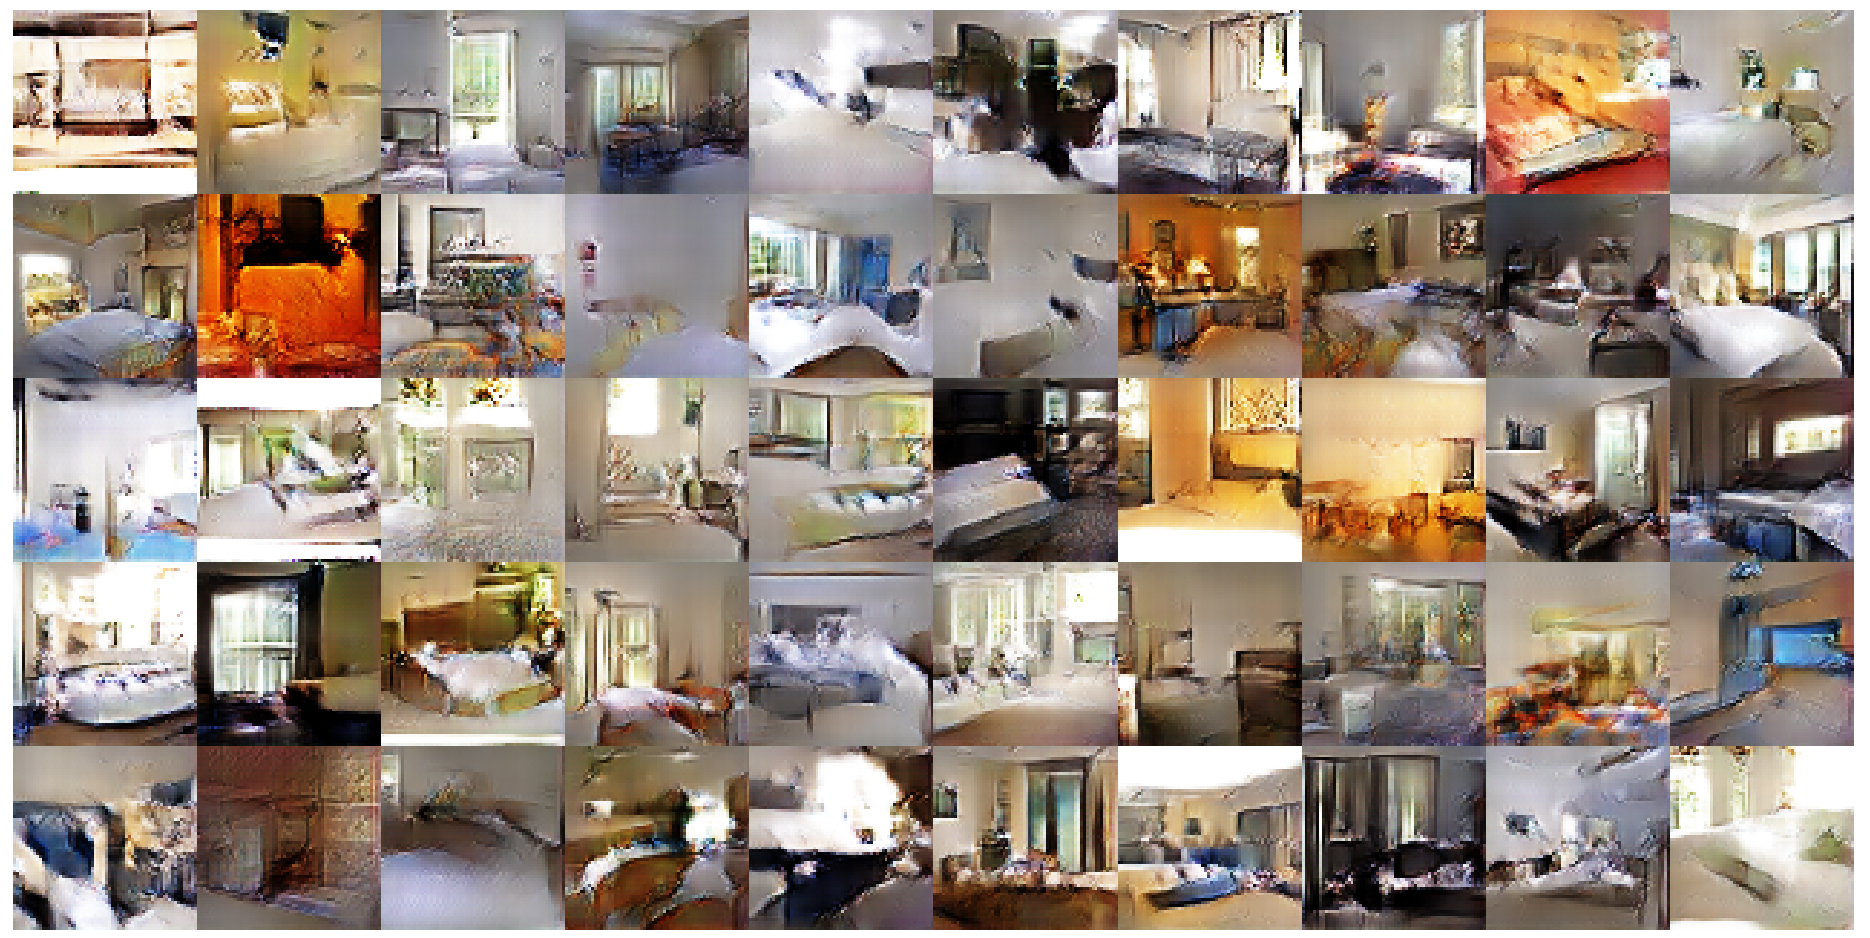
\includegraphics[width=.9\linewidth]{interiers.png}
\end{center}
\end{frame}

\begin{frame}{Интерполяция}
\begin{center}
	\centering	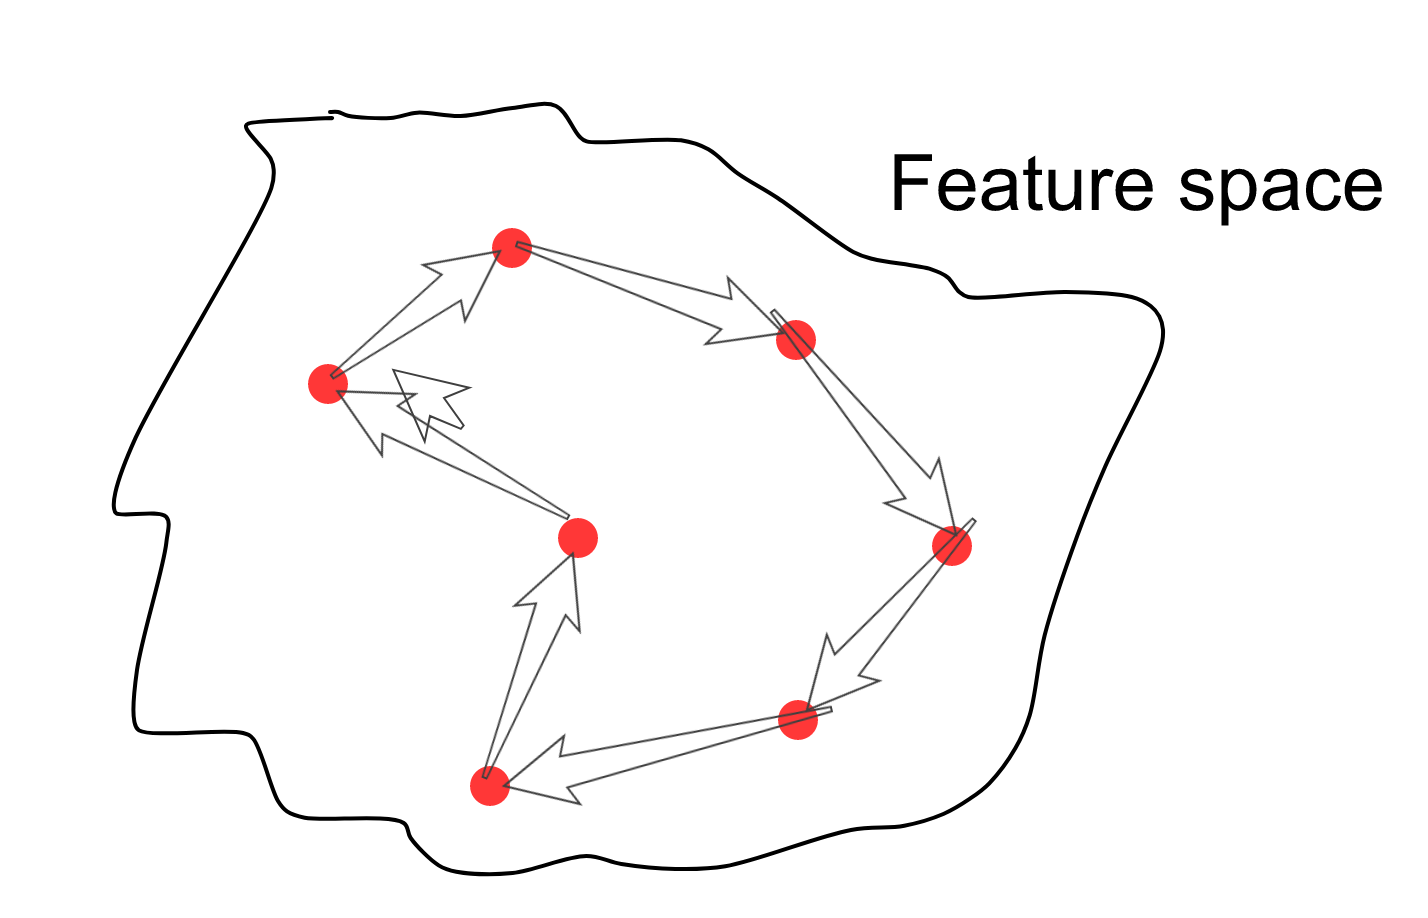
\includegraphics[width=.7\linewidth]{latent_space.png}
\end{center}
\end{frame}

\begin{frame}{Интерполяция}
\begin{center}
\centering	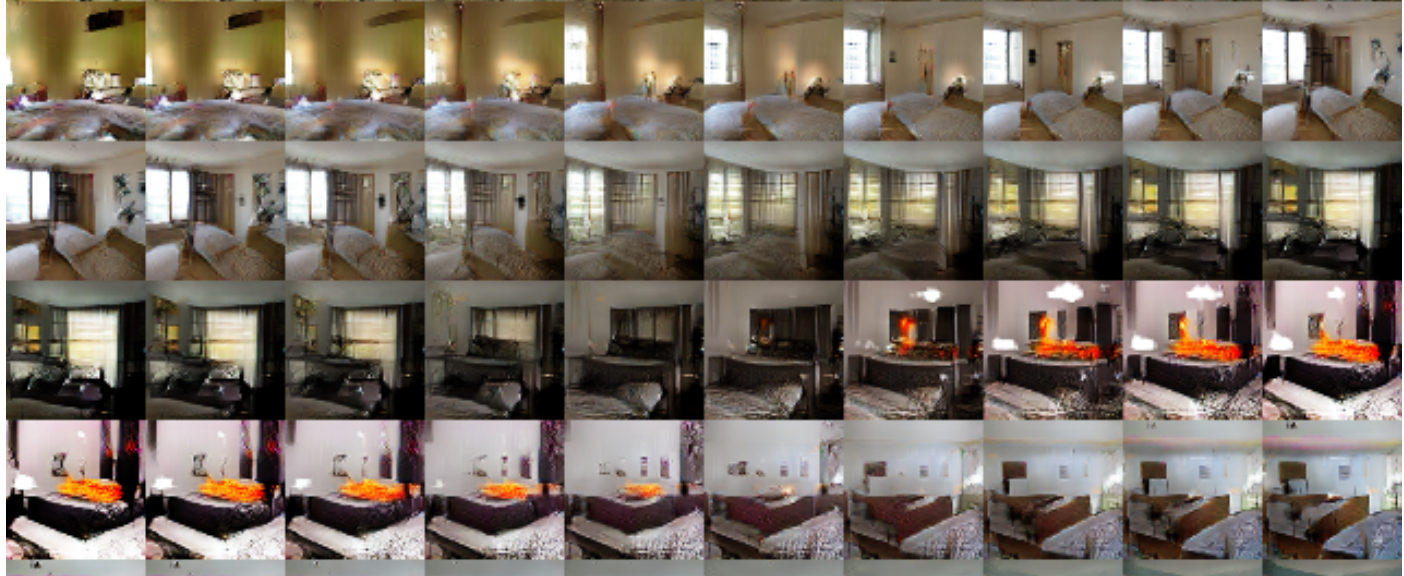
\includegraphics[width=.9\linewidth]{inter1.png}
\end{center}
\end{frame}

\begin{frame}{Интерполяция}
\begin{center}
\centering	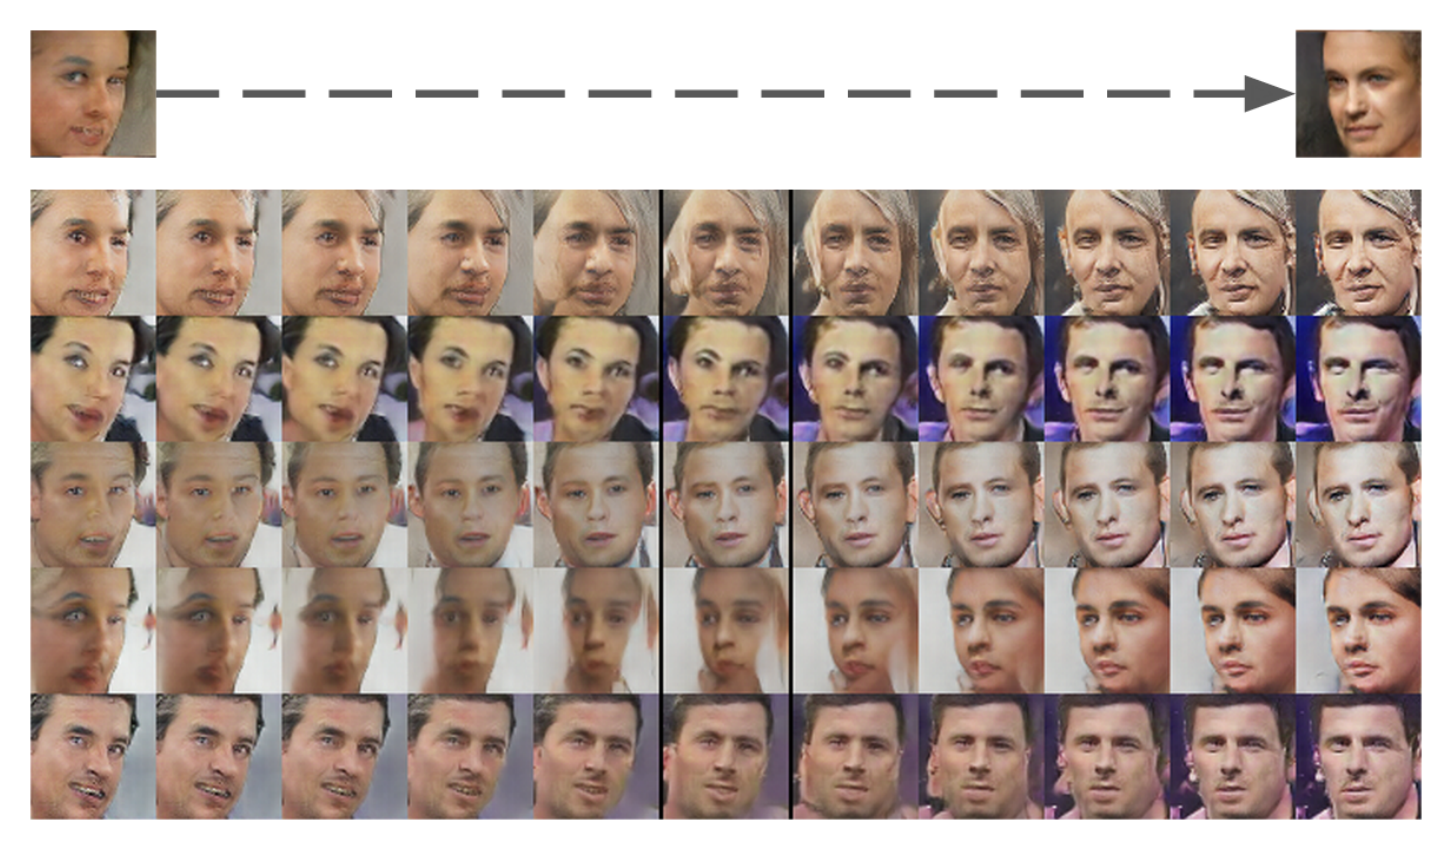
\includegraphics[width=.9\linewidth]{inter2.png}
\end{center}
\end{frame}

\begin{frame}{Арифметика}
\begin{center}
\centering	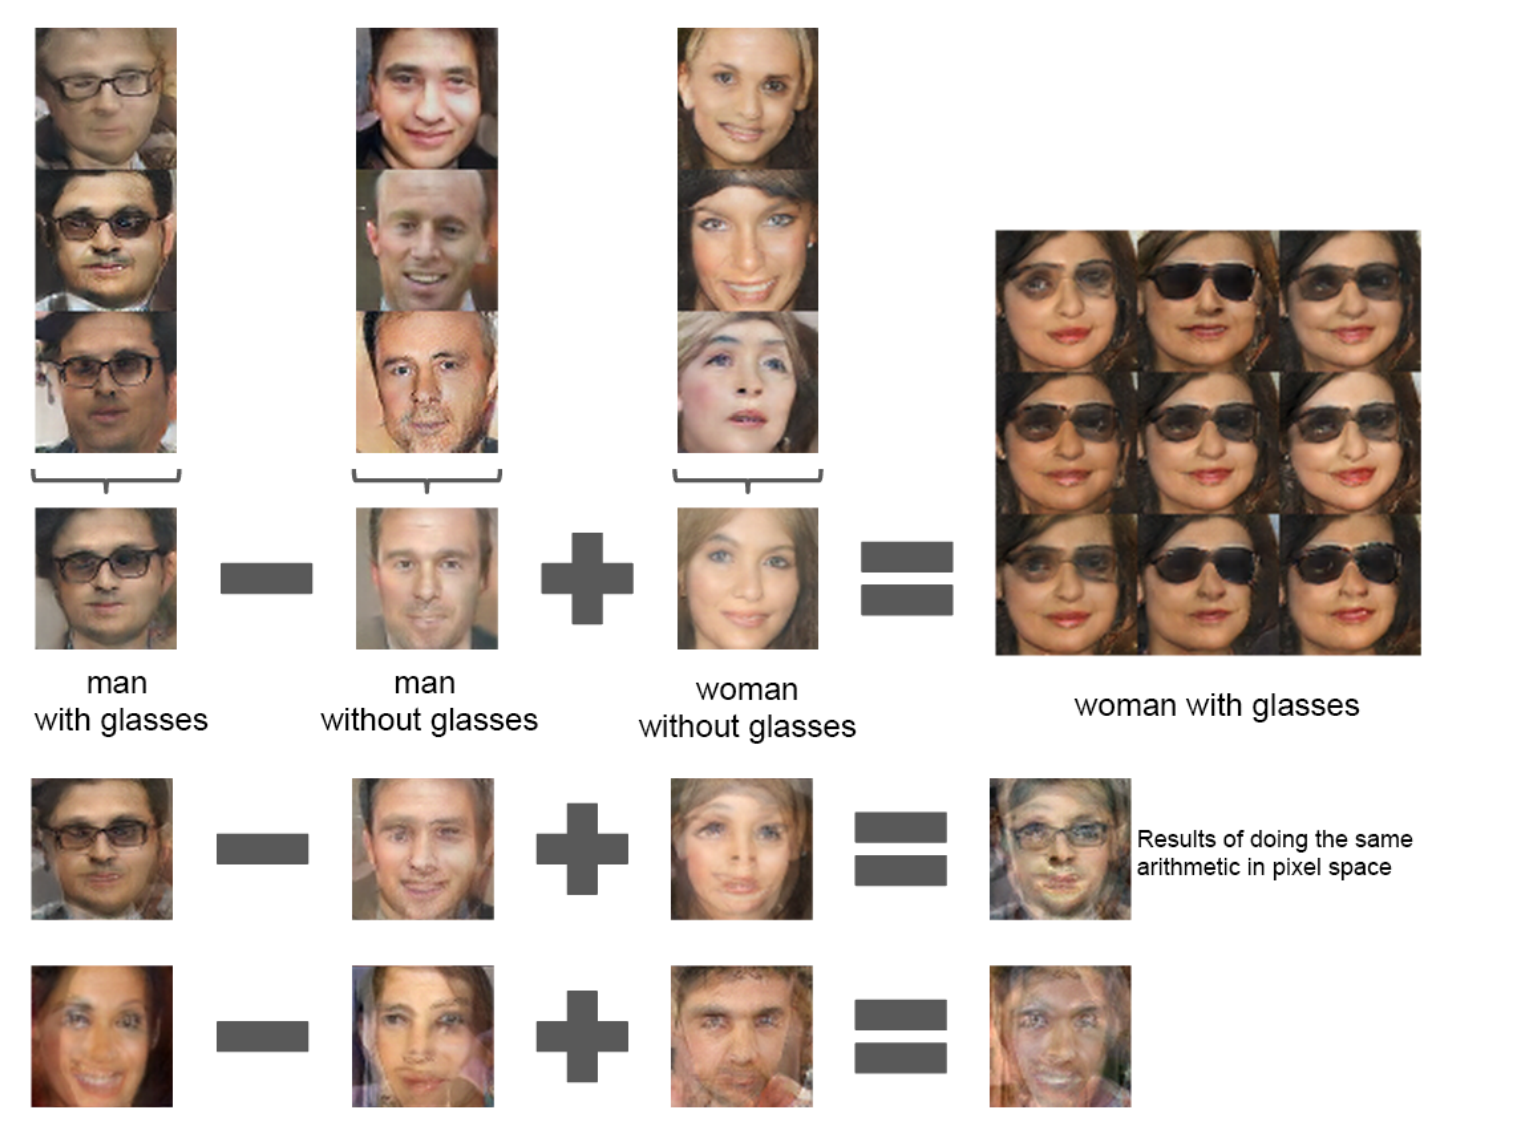
\includegraphics[width=.6\linewidth]{arith.png}
\end{center}
\end{frame}




%\begin{frame}{Примеры драконов}
%\begin{center}
%	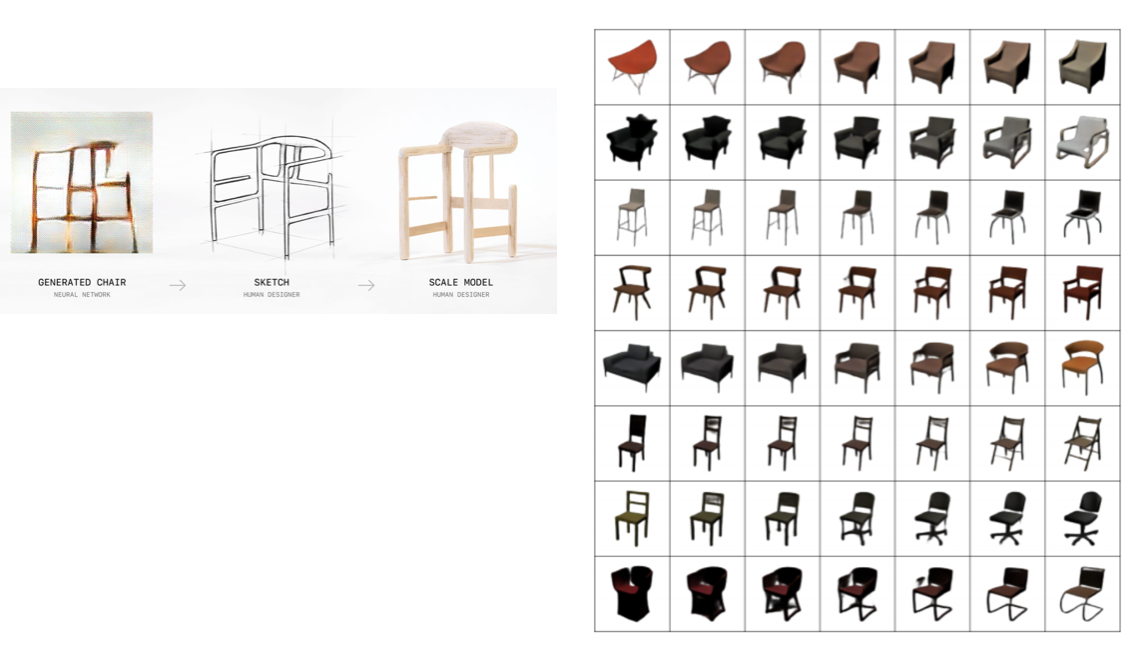
\includegraphics[width=.7\linewidth]{ch_teaser.png}
%\end{center}
%\vfill
%\footnotesize
%{\color{blue} \url{https://rb.ru/story/chair-design/}  \newline 
%\url{https://arxiv.org/pdf/1411.5928.pdf}}
%\end{frame}




\begin{transitionframe}
	\begin{center}
		\Huge  Зоопарк из ганов
	\end{center}
\end{transitionframe}


\begin{frame}{Зоопарк из ганов}
\begin{center}
	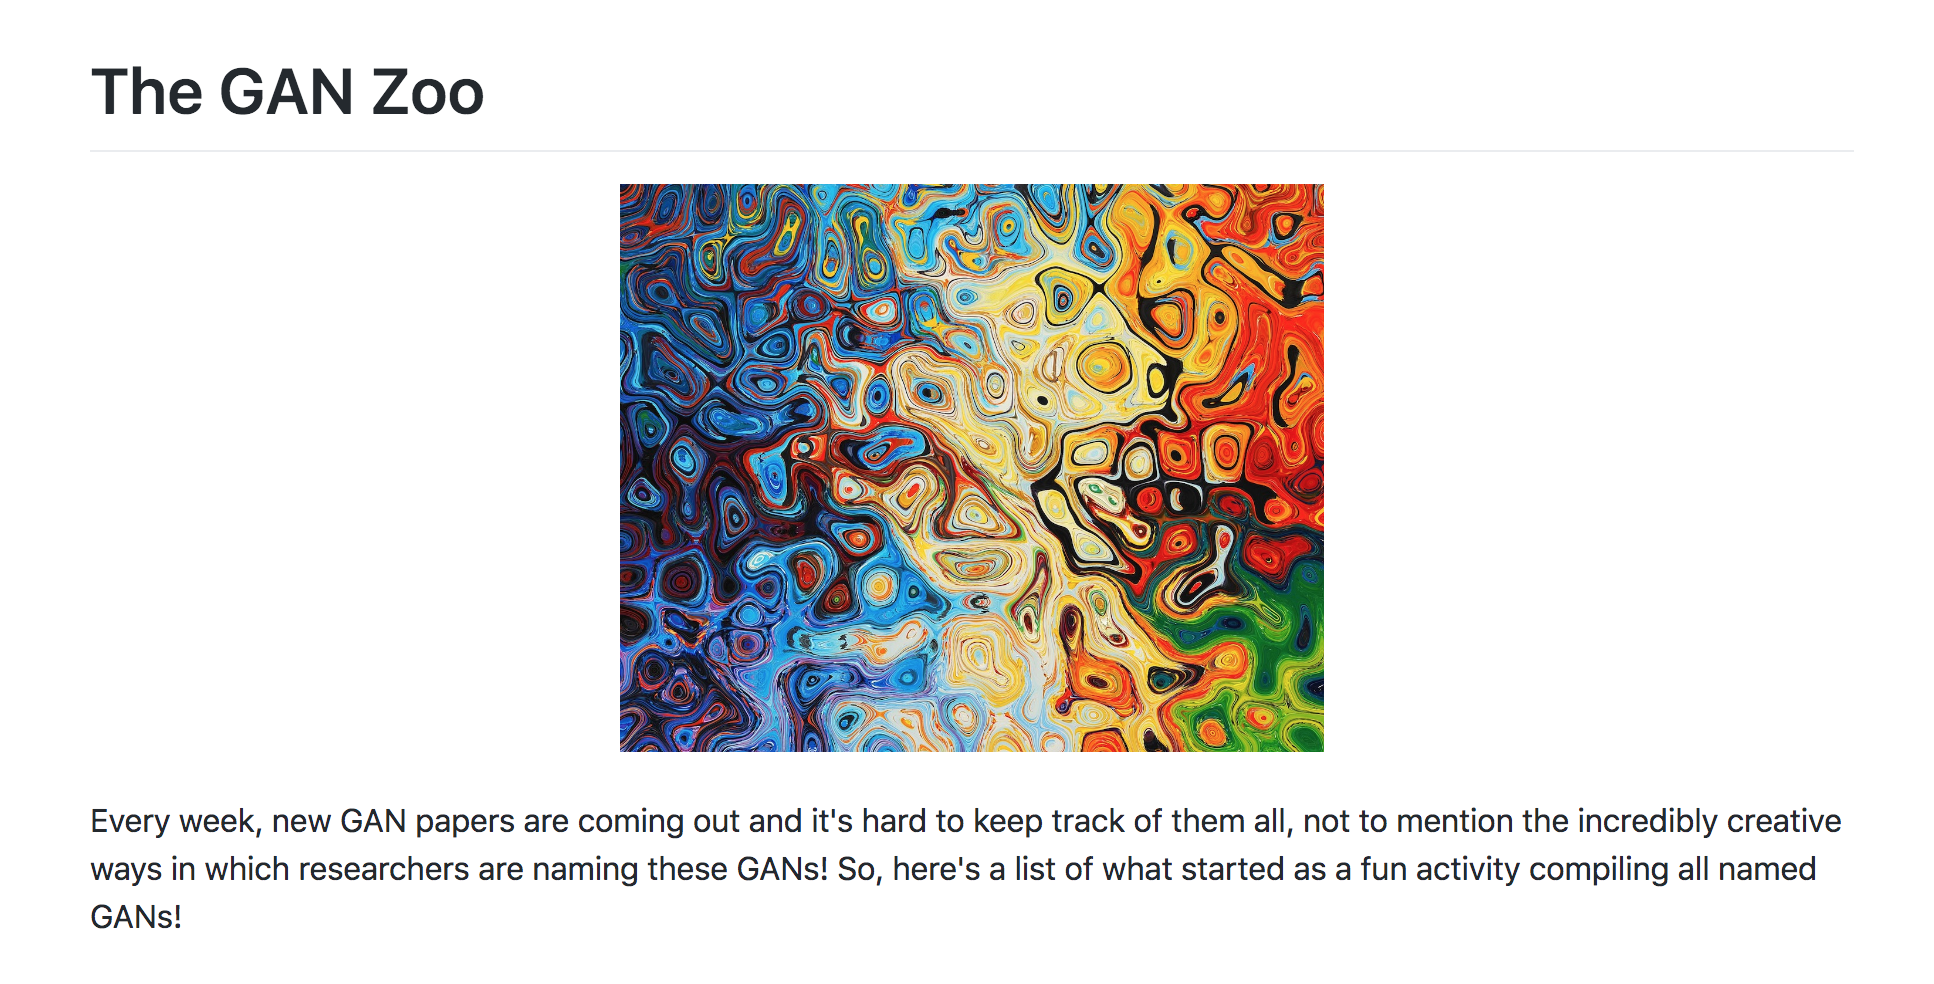
\includegraphics[width=.8\linewidth]{gan_zoo.png}
\end{center}
\vfill
\footnotesize
{\color{blue} \url{https://github.com/hindupuravinash/the-gan-zoo} }
\end{frame}

\begin{frame}{Conditional GAN}
\begin{center}
	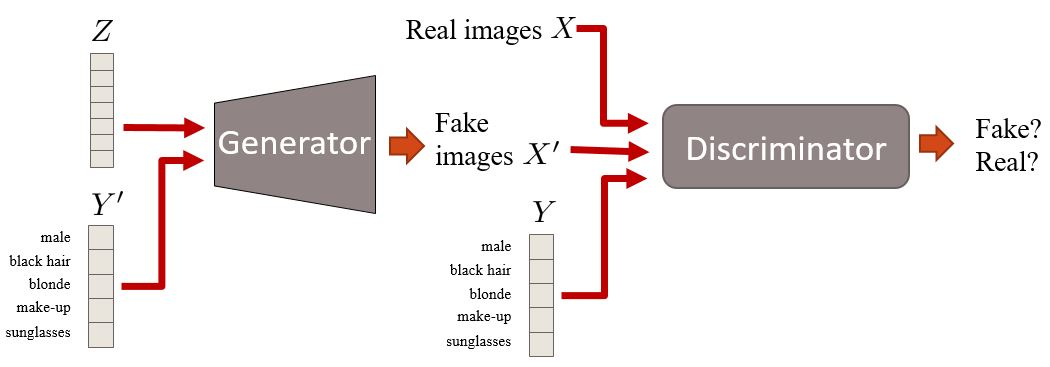
\includegraphics[width=.8\linewidth]{cgan.jpeg}
\end{center}
\vfill
\footnotesize
{\color{blue} \url{https://arxiv.org/pdf/1411.1784.pdf}}
\end{frame}

\begin{frame}{Conditional GAN}
\begin{wideitemize}
	\item   CGAN использует информацию из меток, если они есть
	\item   Это позволяет генерировать не рандомные объекты, а конкретные 
	\item   В качестве меток $y$ можно пытаться использовать и разную другую информацию
	\item   Например, в случае лиц, можно использовать цвет волос, наличие очков, эмоции на лице и тп 
	\item   Можно даже завести несколько разных меток 
\end{wideitemize}
\end{frame}

\begin{frame}{Conditional GAN}
\begin{center}
	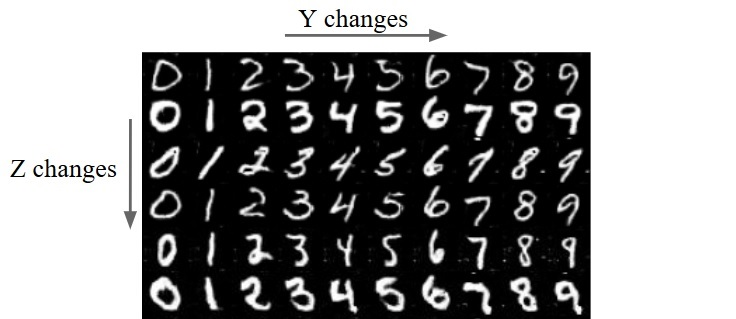
\includegraphics[width=.8\linewidth]{cgan_example.jpeg}
\end{center}
\end{frame}


\begin{frame}{Pix2Pix GAN}
\begin{center}
	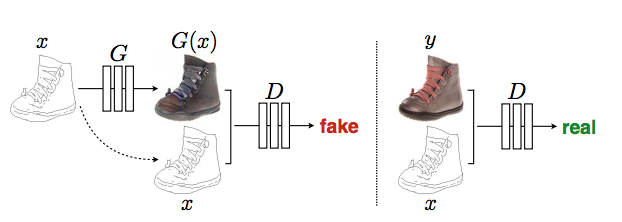
\includegraphics[width=.9\linewidth]{pix2pix_model.png}
\end{center}
\vfill
\footnotesize
{\color{blue} \url{https://arxiv.org/pdf/1808.06601.pdf} \\ 
	\url{https://www.tensorflow.org/tutorials/generative/cyclegan}}
\end{frame}


\begin{frame}{Pix2Pix GAN}
\begin{center}
	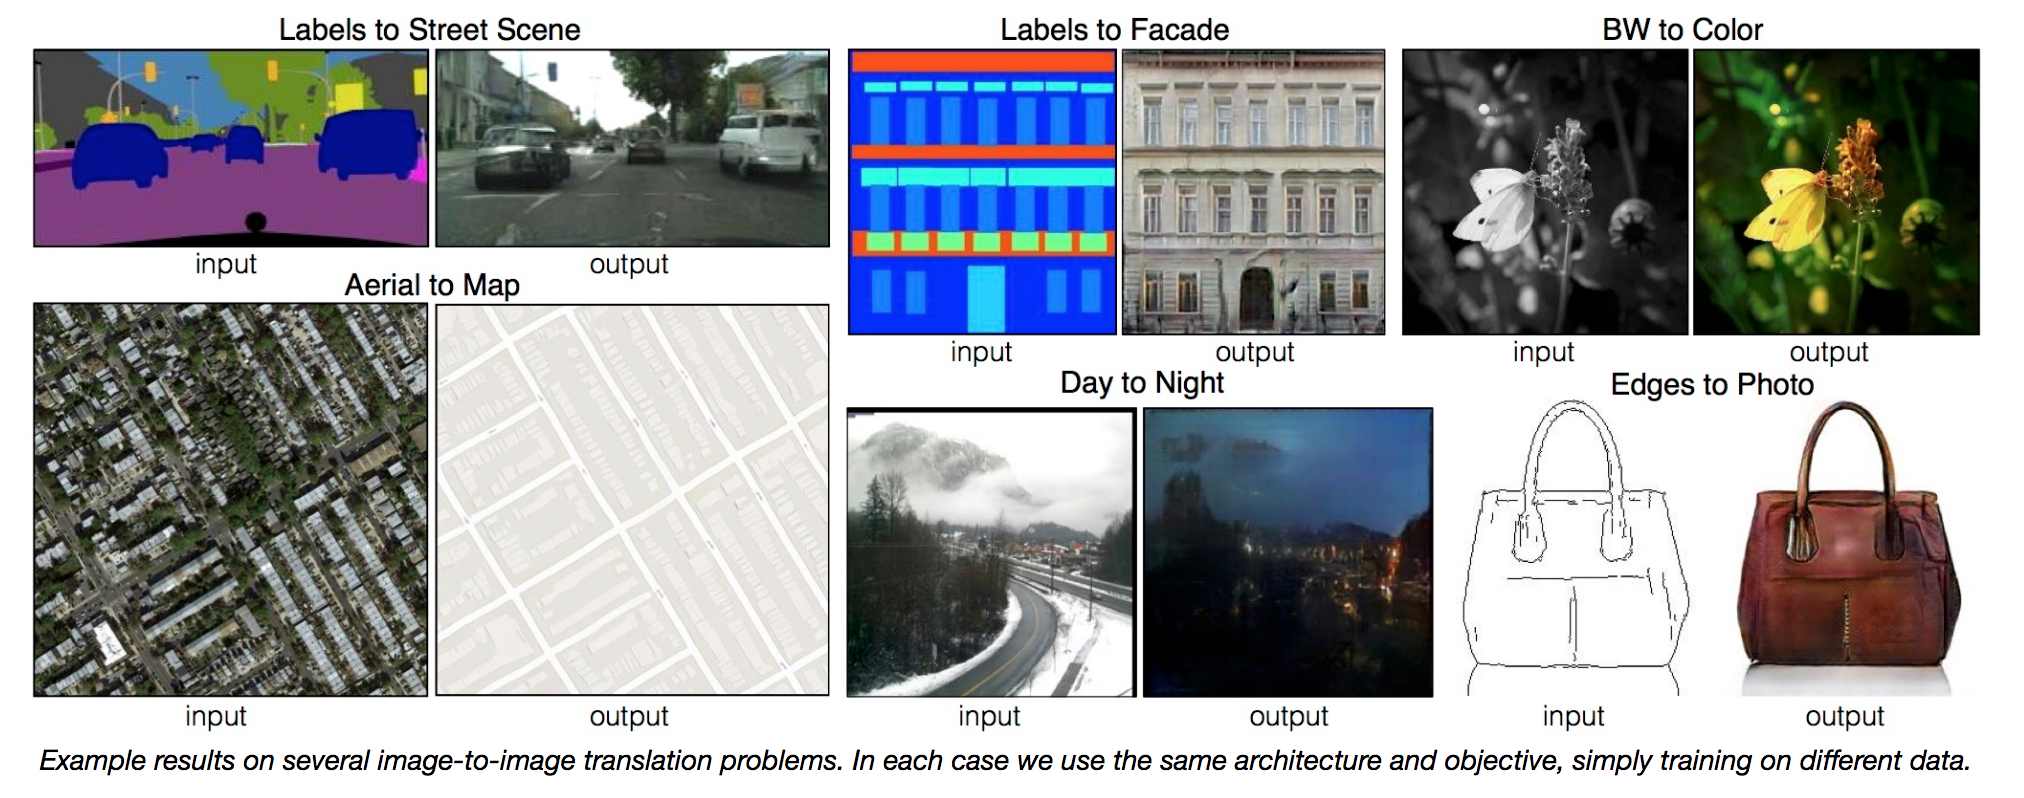
\includegraphics[width=.9\linewidth]{pix2pix.png}
\end{center}
\vfill
\footnotesize
{\color{blue} \url{https://phillipi.github.io/pix2pix/} \\
 \url{https://www.tensorflow.org/tutorials/generative/pix2pix}}
\end{frame}

\begin{frame}{Pix2Pix GAN}
\begin{center}
	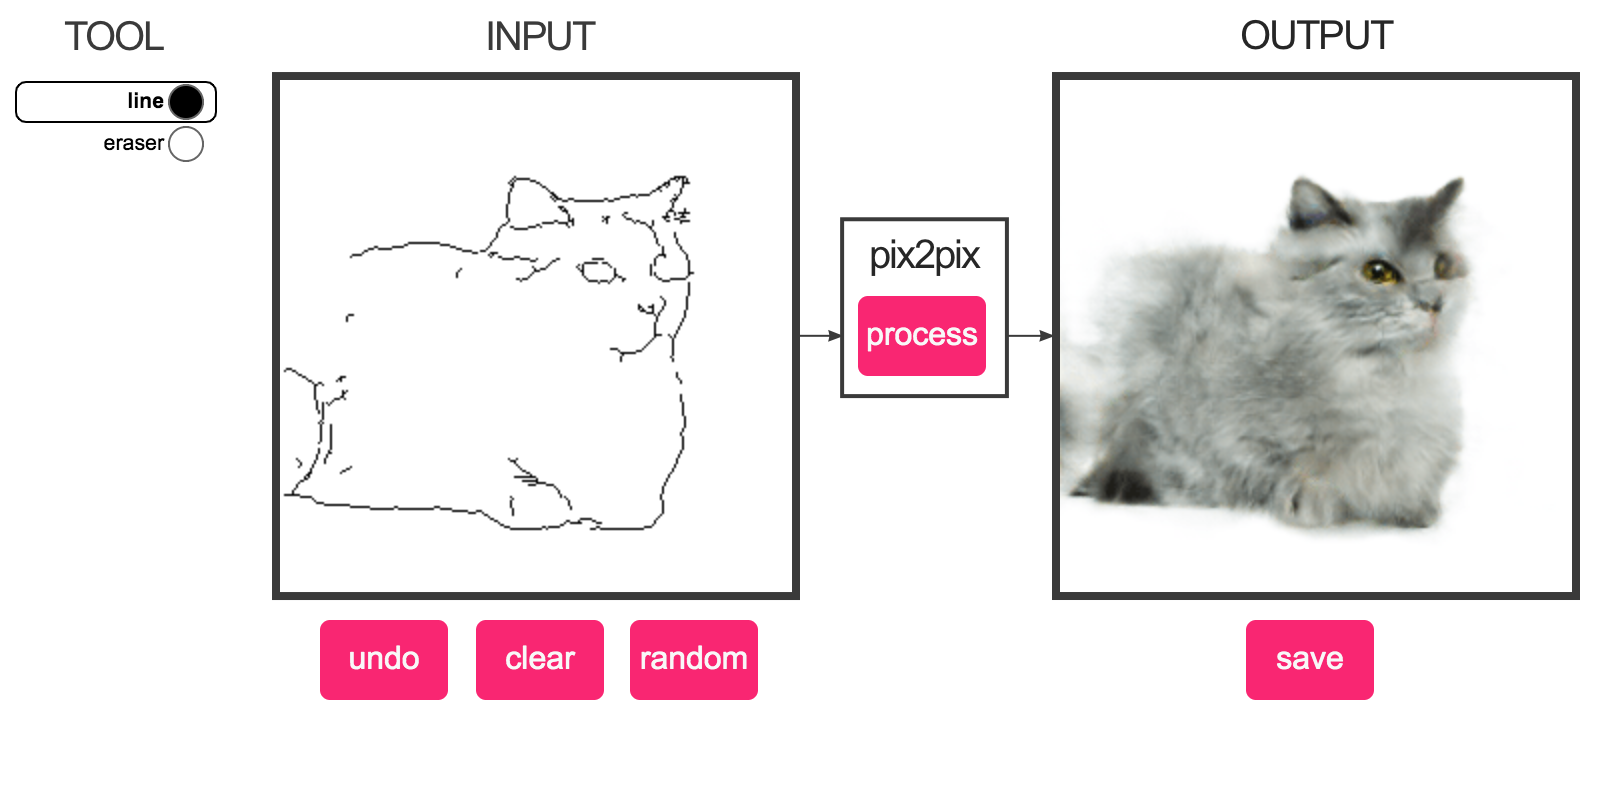
\includegraphics[width=.9\linewidth]{pp.png}
\end{center}
\vfill
\footnotesize
{\color{blue} \url{https://affinelayer.com/pixsrv/}}
\end{frame}

\begin{frame}{Pix2Pix GAN}
\begin{center}
	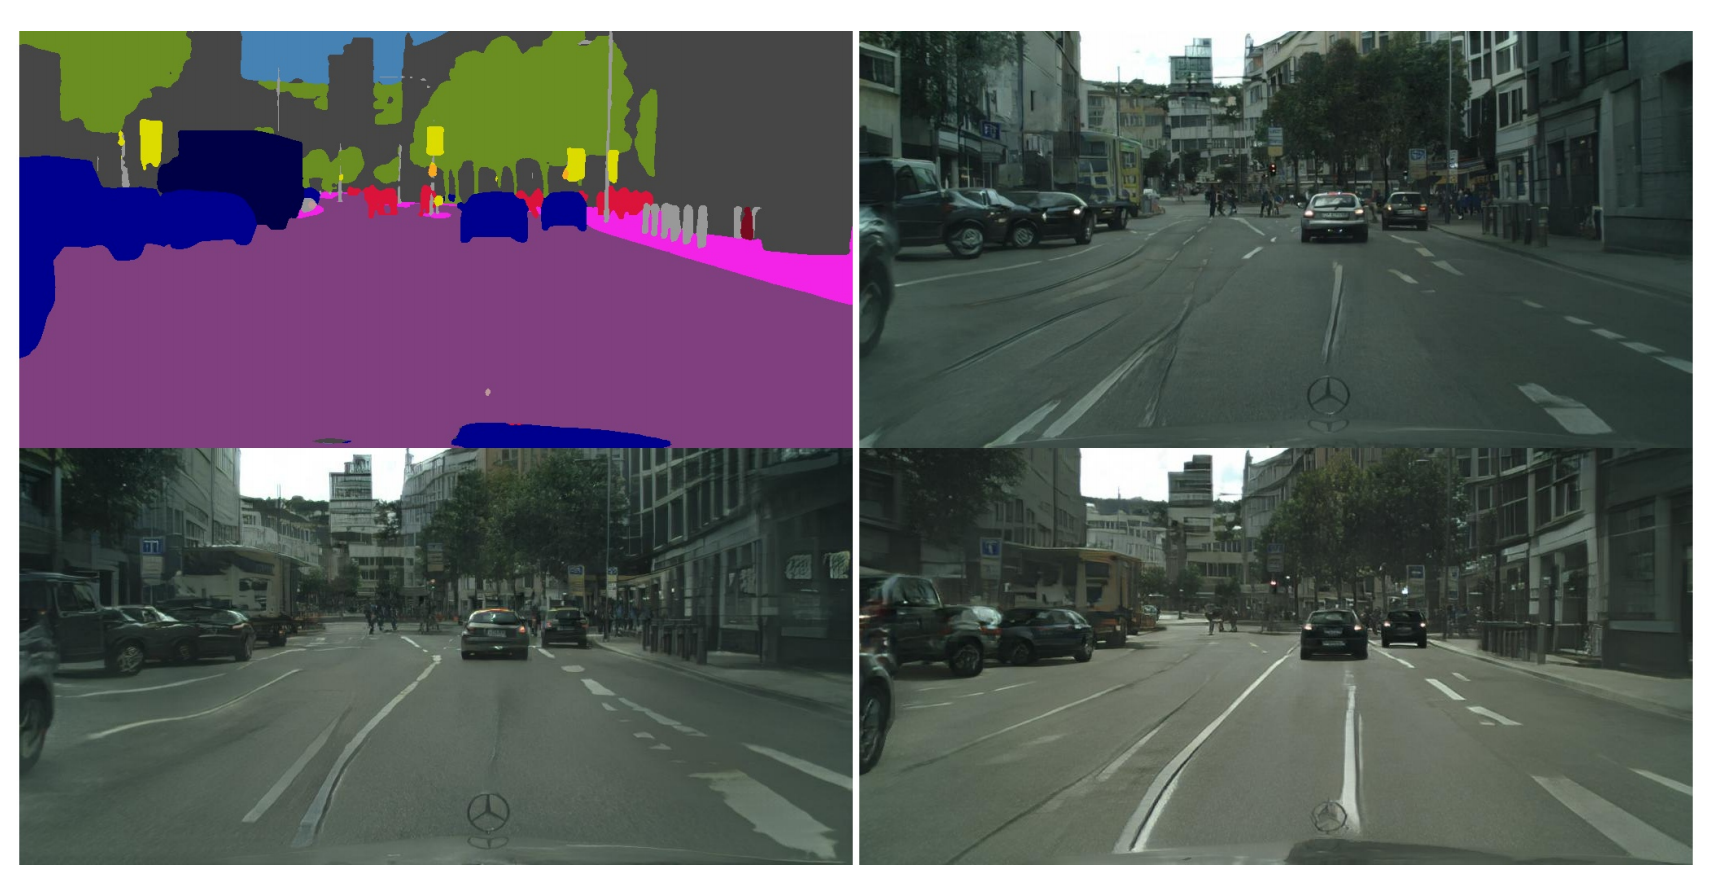
\includegraphics[width=.85\linewidth]{video.png}
\end{center}
\end{frame}


\begin{frame}{CycleGAN}
\begin{center}
	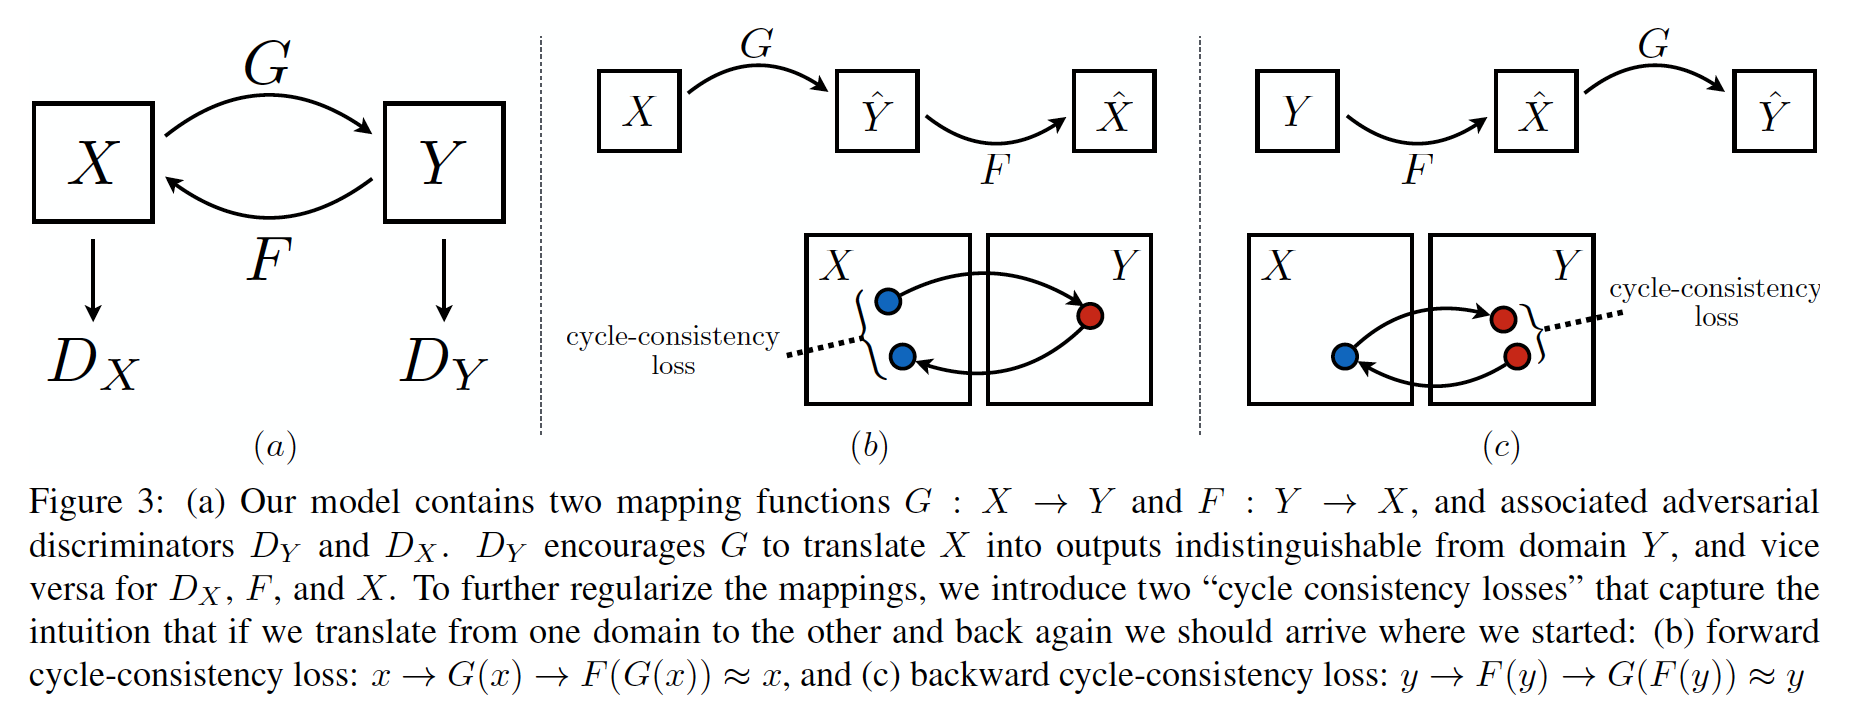
\includegraphics[width=.9\linewidth]{cyclegan.png}
\end{center}
\vfill
\footnotesize
{\color{blue} \url{https://arxiv.org/abs/1703.10593}} \\ 
{\color{blue} \url{https://www.tensorflow.org/tutorials/generative/cyclegan}} 
\end{frame}

\begin{frame}{Conditional GAN}
\begin{wideitemize}
	\item   $X$ — объекты первого типа, $Y$ — объекты второго типа 
	\item   Два генератора, у каждого свой дискриминатор 
	\item   Дискриминатор пытается понять правильный $X$ пришёл на вход или он сделан из $Y$ 
	\item   Сетки генераторы сделаем обратными друг к другу функциями
\end{wideitemize}
\end{frame}

\begin{frame}{CycleGAN}
\begin{center}
	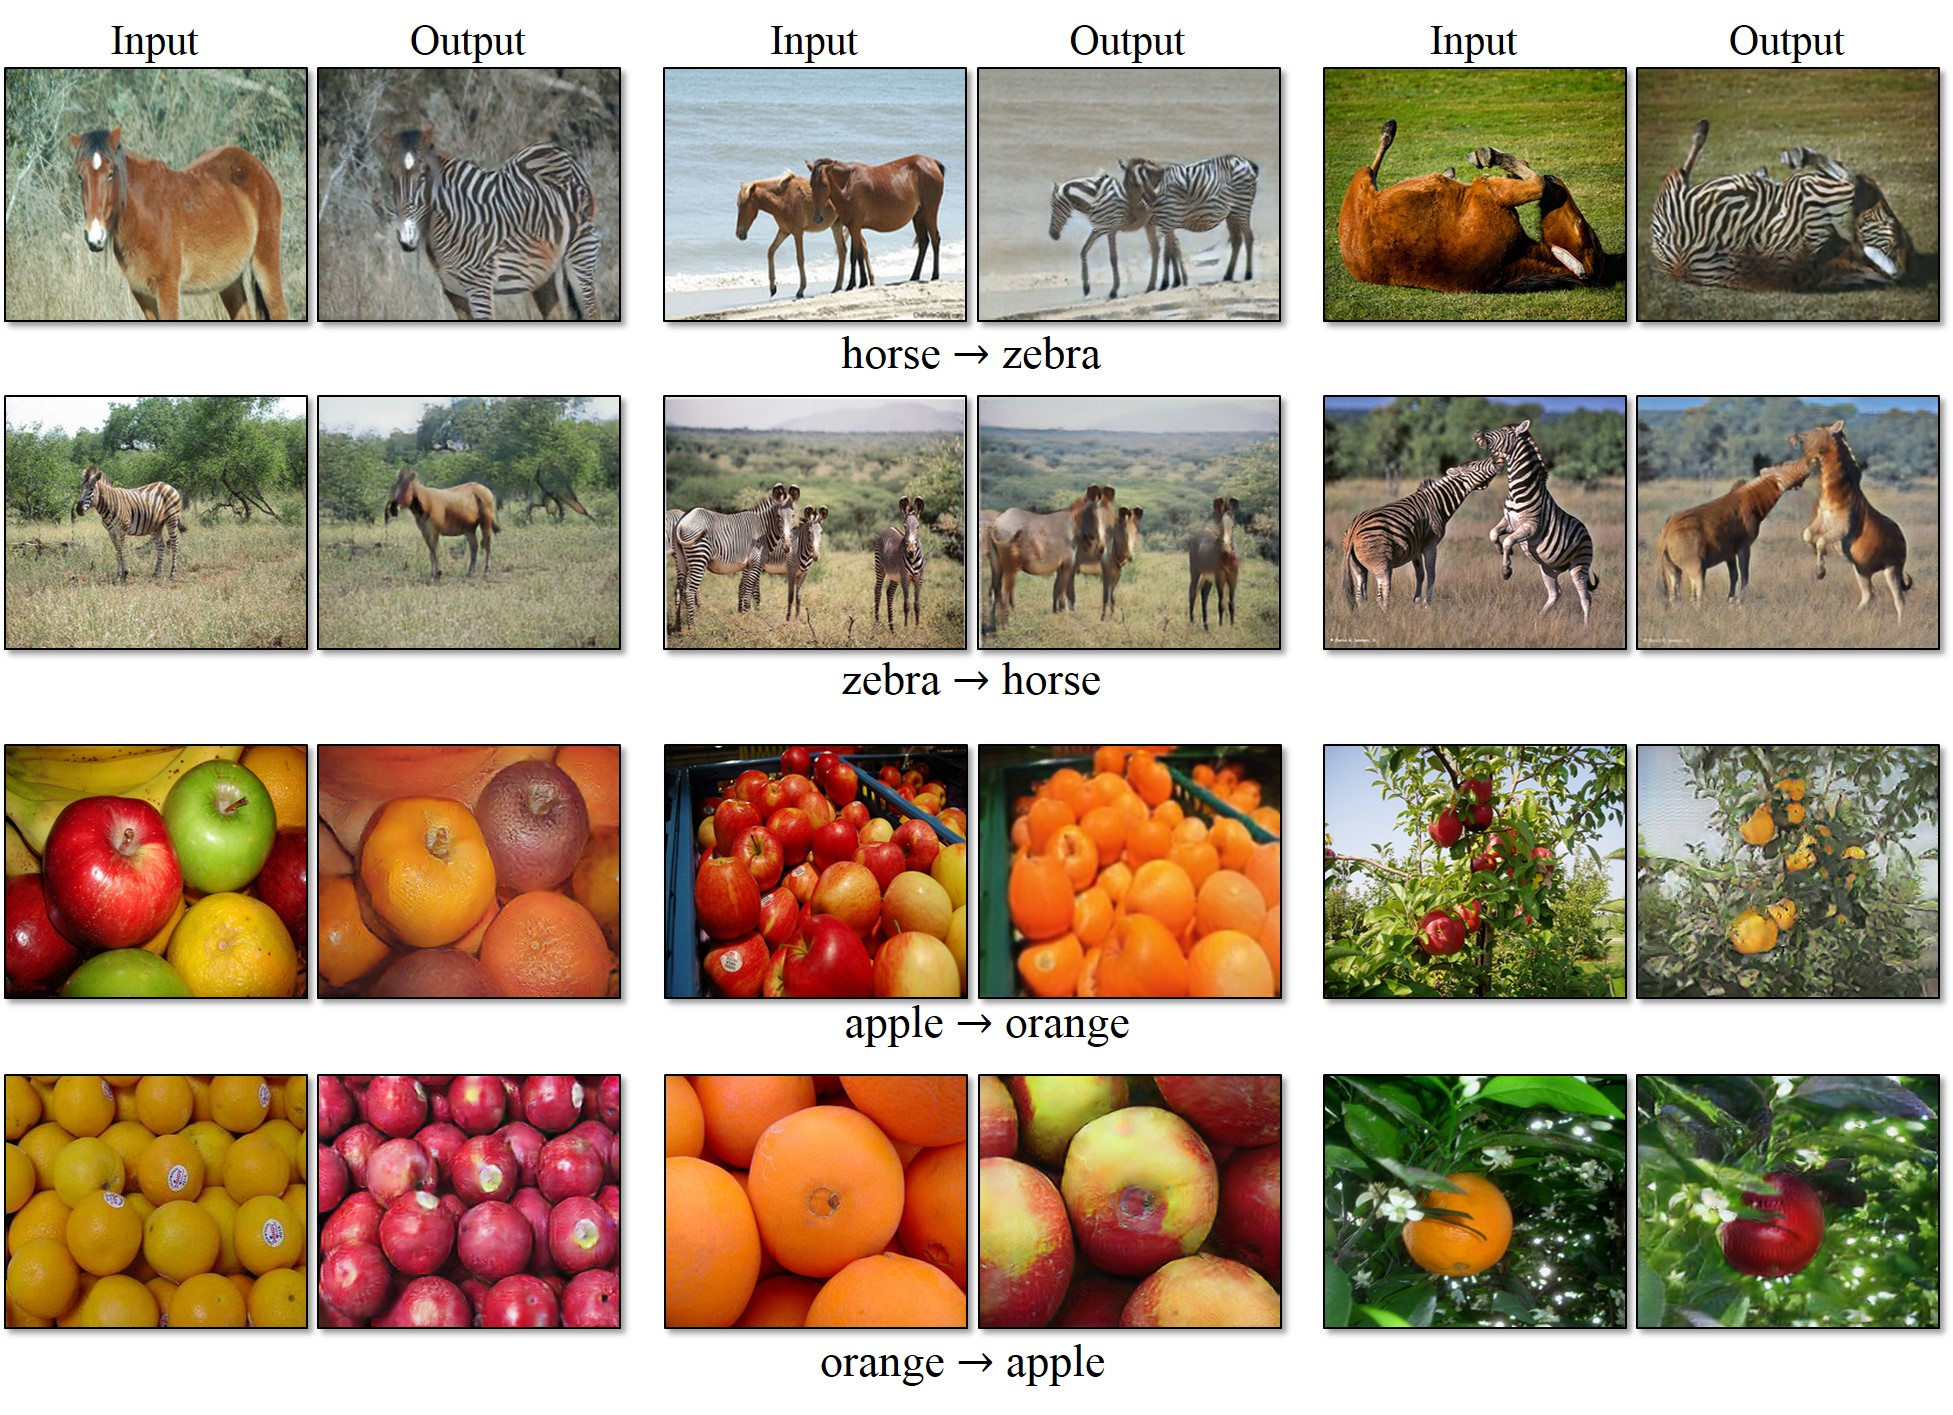
\includegraphics[width=.7\linewidth]{cycle_gan.jpg}
\end{center}
\end{frame}

\begin{frame}{Почиташки}
\begin{wideitemize}
	\item   {\color{blue}  \href{https://habr.com/ru/company/ods/blog/322514/}{Отличный обзор} }  разных статеек про GAN на хабре, от оригинальной статьи до продвинутых идей 
	
	\item   {\color{blue}  \href{https://habr.com/ru/post/331382/}{{Хорошая серия статей}}} про ганы и автокодировщики 
	
	\item    {\color{blue}  \href{https://drive.google.com/file/d/1TLgtJYIs7hmDwrjbqhCjCrVmGUbc6orI/view}{Отлично написанная глава про GAN }} из уже ставшей классической книги про нейросетки от Николенко 
		
	\item   {\color{blue}  \href{http://nightmare.mit.edu/}{{Генератор хороров}}} от MIT
\end{wideitemize}
\end{frame}


\end{document}
